\section{Path Following}
\label{chap:path_following}
% Explain what should a path follower do and how, then describe how it has been implemented
The first task our controller should accomplish is to follow a reference path.
How this reference path is given to the controller, is described in the Section \ref{chap:SignalAcquisition} - Signal Acquisition, where we assume that we have an high level device which is able to provide to the controller a sampled map composed by a sequence of waypoints reporting $x$, $y$, $\theta$, and $v$ for each timestep of the control. We pass to the controller the next \textit{p} steps in the reference map, where \textit{p} is the number of steps of the prediction horizon.\\
Before the final testing process, we have performed several simulations in order to obtain a fine controller tuning regarding its weights, relative to output variables and manipulated variables, and other influential quantities. \\
The best results for path following are achieved with the following configuration:
\begin{table}[H]
\centering
\begin{tabular}{|l|r|}\hline
Sample Time                        & 0.01 s           \\ \hline
Prediction Horizon                 & 15 steps         \\ \hline
Control Horizon                    & 5 steps          \\ \hline
Output Variables Weights           & {[}30 30 8 30{]} \\ \hline
Manipulated Variables Weights      & {[}0 0{]}        \\ \hline
Manipulated Variables Rate Weights & {[}0 0{]}       \\ \hline
\end{tabular}
\caption{Configuration parameters adopted for Path Following}
\label{tab:configuration}
\end{table}
For the sake of the Path Following task, only the constraints on the inputs are considered, neglecting any constraint on the states.\\
Moreover, we have set the initial value for the \textit{covariance matrix} of the internal state estimator to $\left[ \begin{smallmatrix} 1000 & 0 & 0 & 0 & 0 & 0 \\0 & 1000 & 0 & 0 & 0 & 0 \\0 & 0 & 1000 & 0 & 0 & 0 \\ 0 & 0 & 0 & 1000 & 0 & 0 \\ 0 & 0 & 0 & 0 & 1000 & 0 \\ 0 & 0 & 0 & 0 & 0 & 1000 \end{smallmatrix} \right] $ to avoid oscillations in the starting phase of the control, due to the discrepancies between the plant model given to the controller and the dynamic plant model used for simulation.
Covariance matrix is $6\times 6$ because it is related to 4 states and 2 inputs.\\
This matrix is automatically updated by the MPC algorithm in runtime.
\subsection{Path Following - Testing} \label{subsection:path_following_testing}
% Describe the tests to validate the path following algorithm
Path following tests aim to evaluate the performance of a path follower in different scenarios with speed ranging from 10 to 100 km/h as stated in Section \ref{System_Requirements} - System Requirements.
In order to satisfy requirements 1 and 5 regarding respectively the \textit{maximum lateral error} and the \textit{maximum lateral acceleration}, we setup a test-bench to assert these quantities. In detail, to verify the lateral error, we built a function to approximate the distance between the actual point in which the vehicle is and the reference trajectory. This function is based on the assumption that the vehicle is close enough to the reference point considered and the reference, in the close proximity of the point itself, can be approximated as a straight line. These considerations are summarized by the following equation:
\begin{equation}
    Lateral\_dev = \frac{\|y_{vehicle} - (mx_{vehicle} + q)\|}{\sqrt{1 + m^2}} \label{eq:lateral_dev}
\end{equation}
where:\\
\begin{center}
 $   m = \tan(\theta_{ref}) $\\ 
 $  q = y_{ref}-mx_{ref}$
\end{center}
\vspace{10pt}
The tests are considered passed if the following conditions are verified:
\begin{itemize}
    \item lateral deviation always lower than 1.0 $m$;
    \item lateral deviation does not exceed 0.75 $m$ for more than 1 $s$.
\end{itemize}
\vspace{10pt}
For what concerns the lateral acceleration we get it directly from the state of the dynamic model as reported in Section \ref{chap:Vehicle_model}, equation \ref{dynamic_equation}: $\ddot{y} = -\dot{\psi}\dot{x} + \frac{2}{m}\left(F_fcos(\delta) + F_r\right)$.\\
The test is considered passed if the lateral acceleration does not exceed 2.0 $m/s^2$ for more than 0.5 $s$.\\ \\
Each path following test has been performed with all the vehicles stored in our database, as reported in section \ref{chap:Vehicle_model} Table \ref{tab:vehicle_data}.

\pagebreak
The scenarios we have selected are the following:
\begin{enumerate}
    \item \textbf{Straight line}: this is the simplest possible scenario, consisting of a straight line starting from $(0,0)$ up to $(1000,0)$ in the X-Y reference frame, with 0° orientation. We repeated this scenario twice with speeds respectively of 10 km/h and 100 km/h;
    \begin{figure}[H]
    \centering
    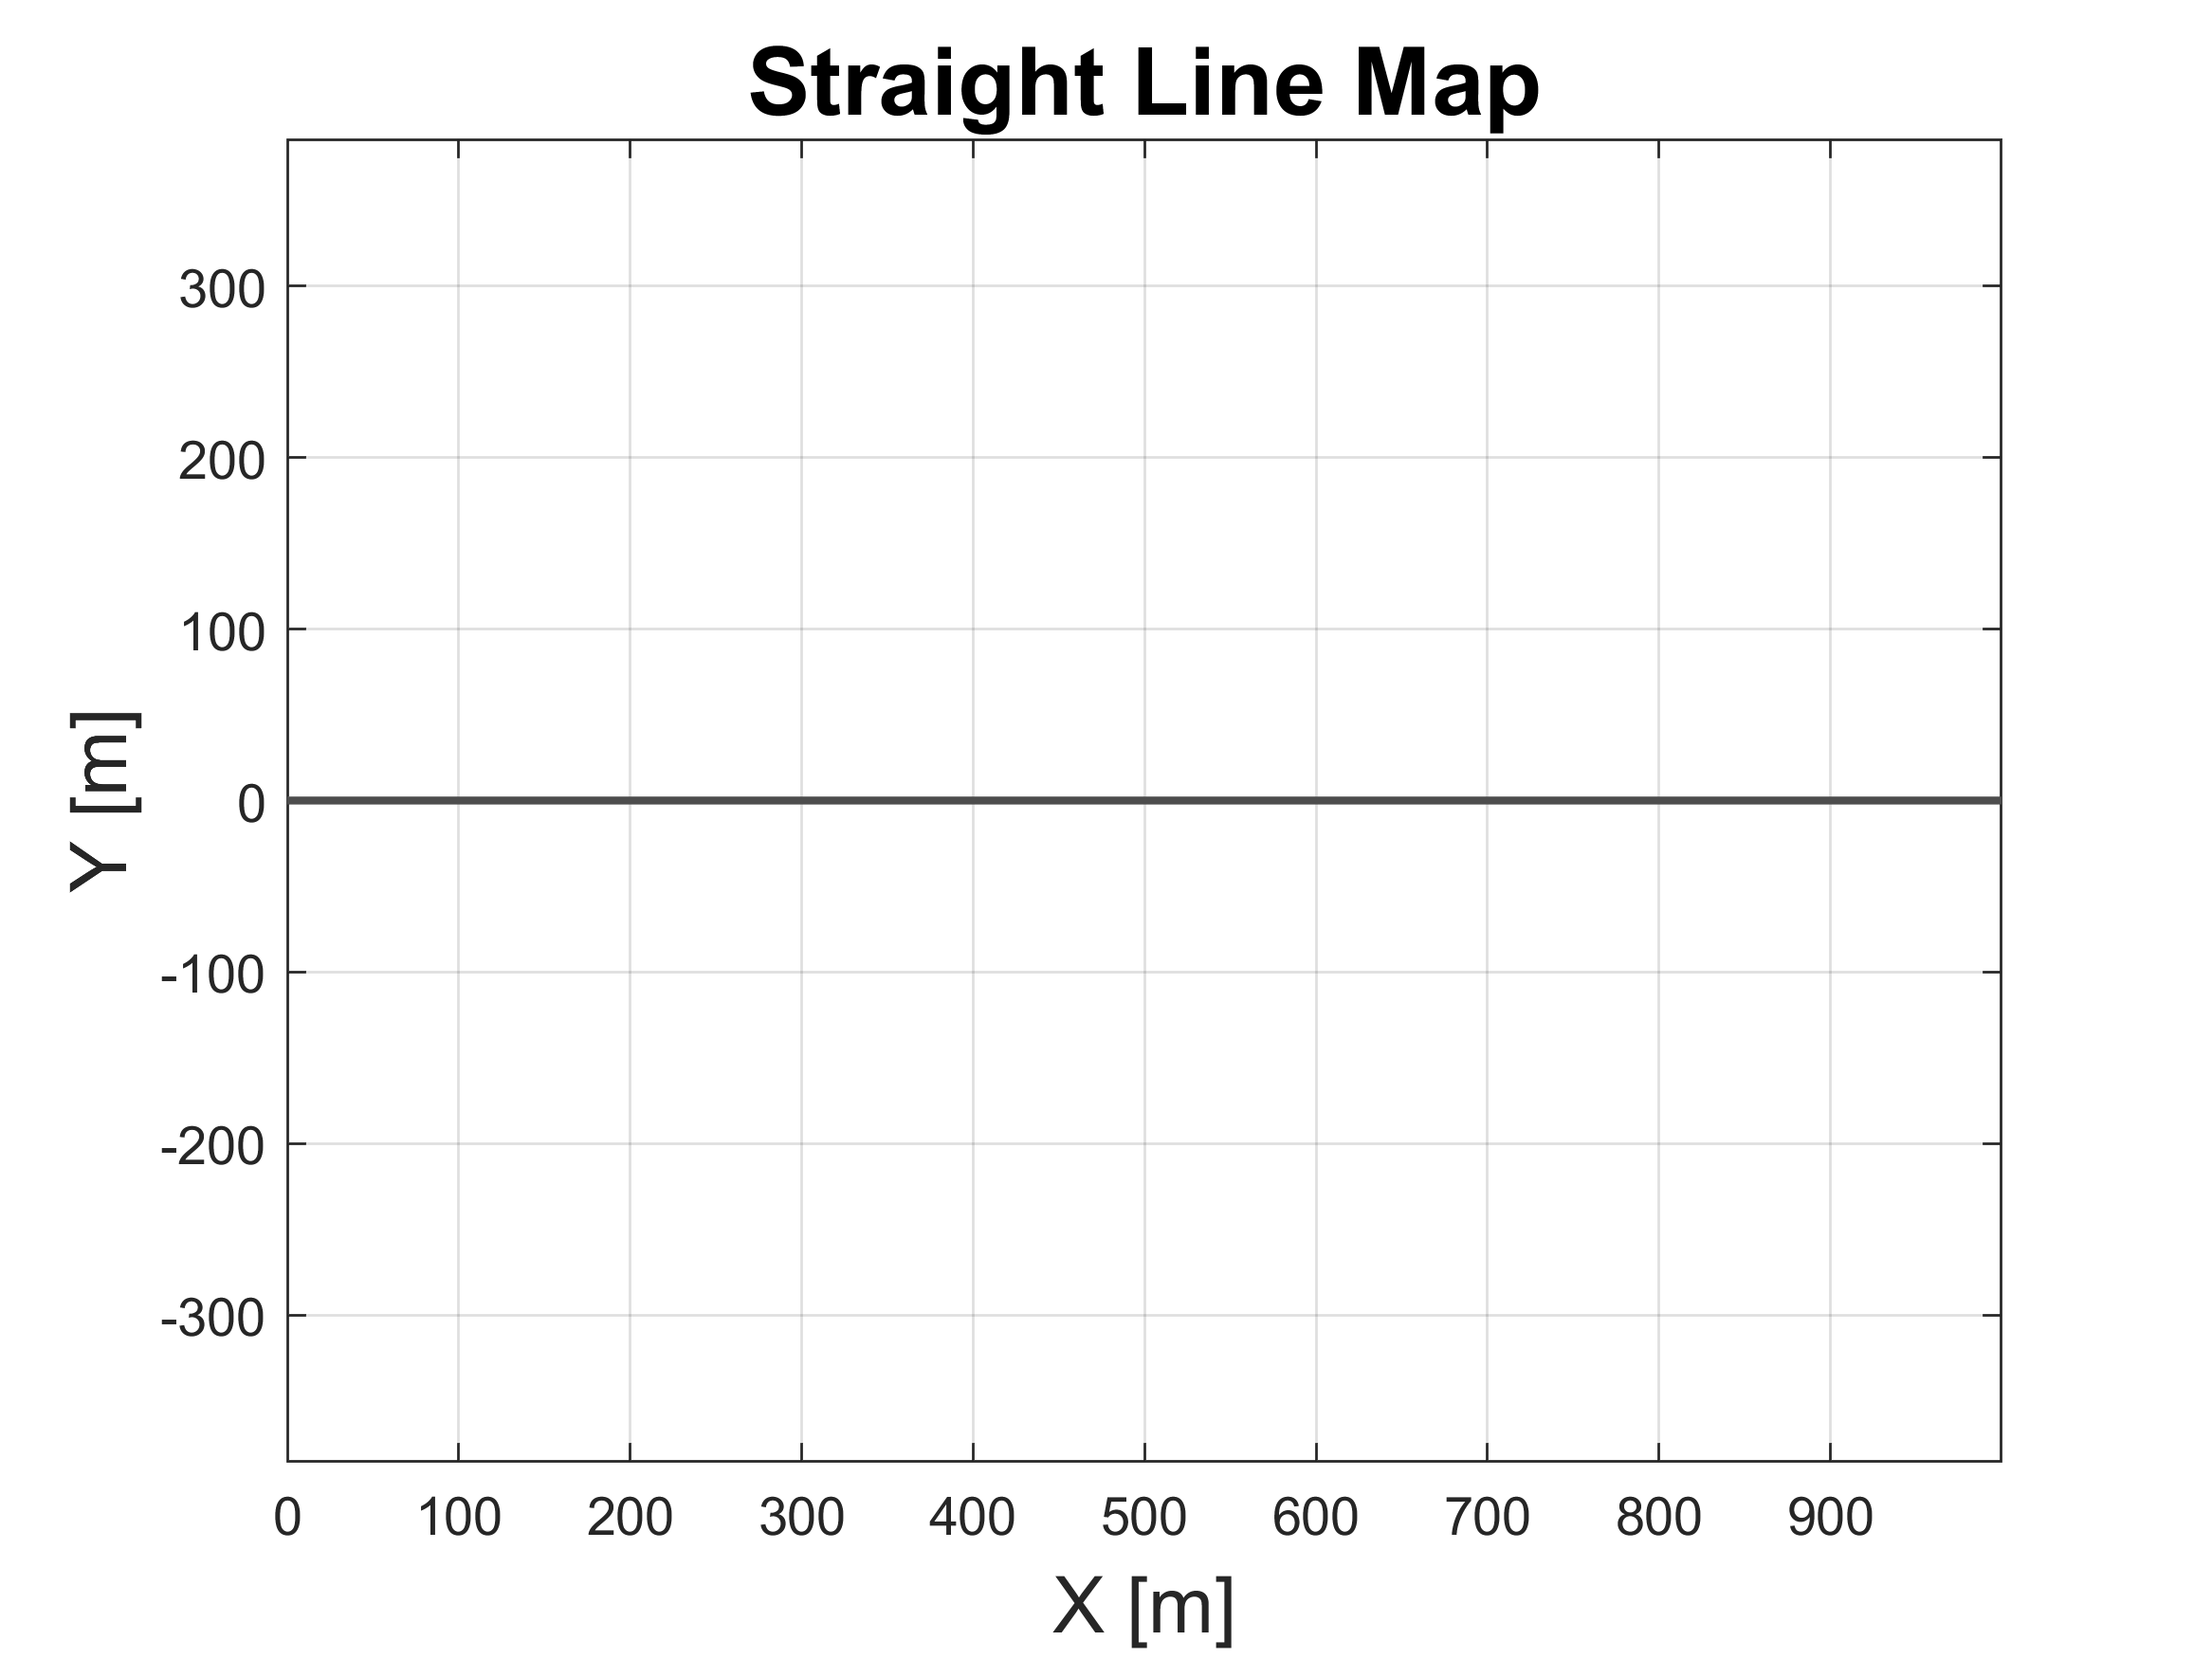
\includegraphics[width=0.7\textwidth]{Figures/StraightMap.png}
    \caption{Straight line Map}
      \label{fig:StraightMap}
\end{figure}
\vspace{1cm}
    \item \textbf{Tilted straight line - 45°}: this is a simple scenario consisting of a straight line starting from $(0,0)$ up to $(1000,1000)$, with an orientation of 45°. We selected a speed of 10 km/h for this scenario;
    \begin{figure}[H]
    \centering
    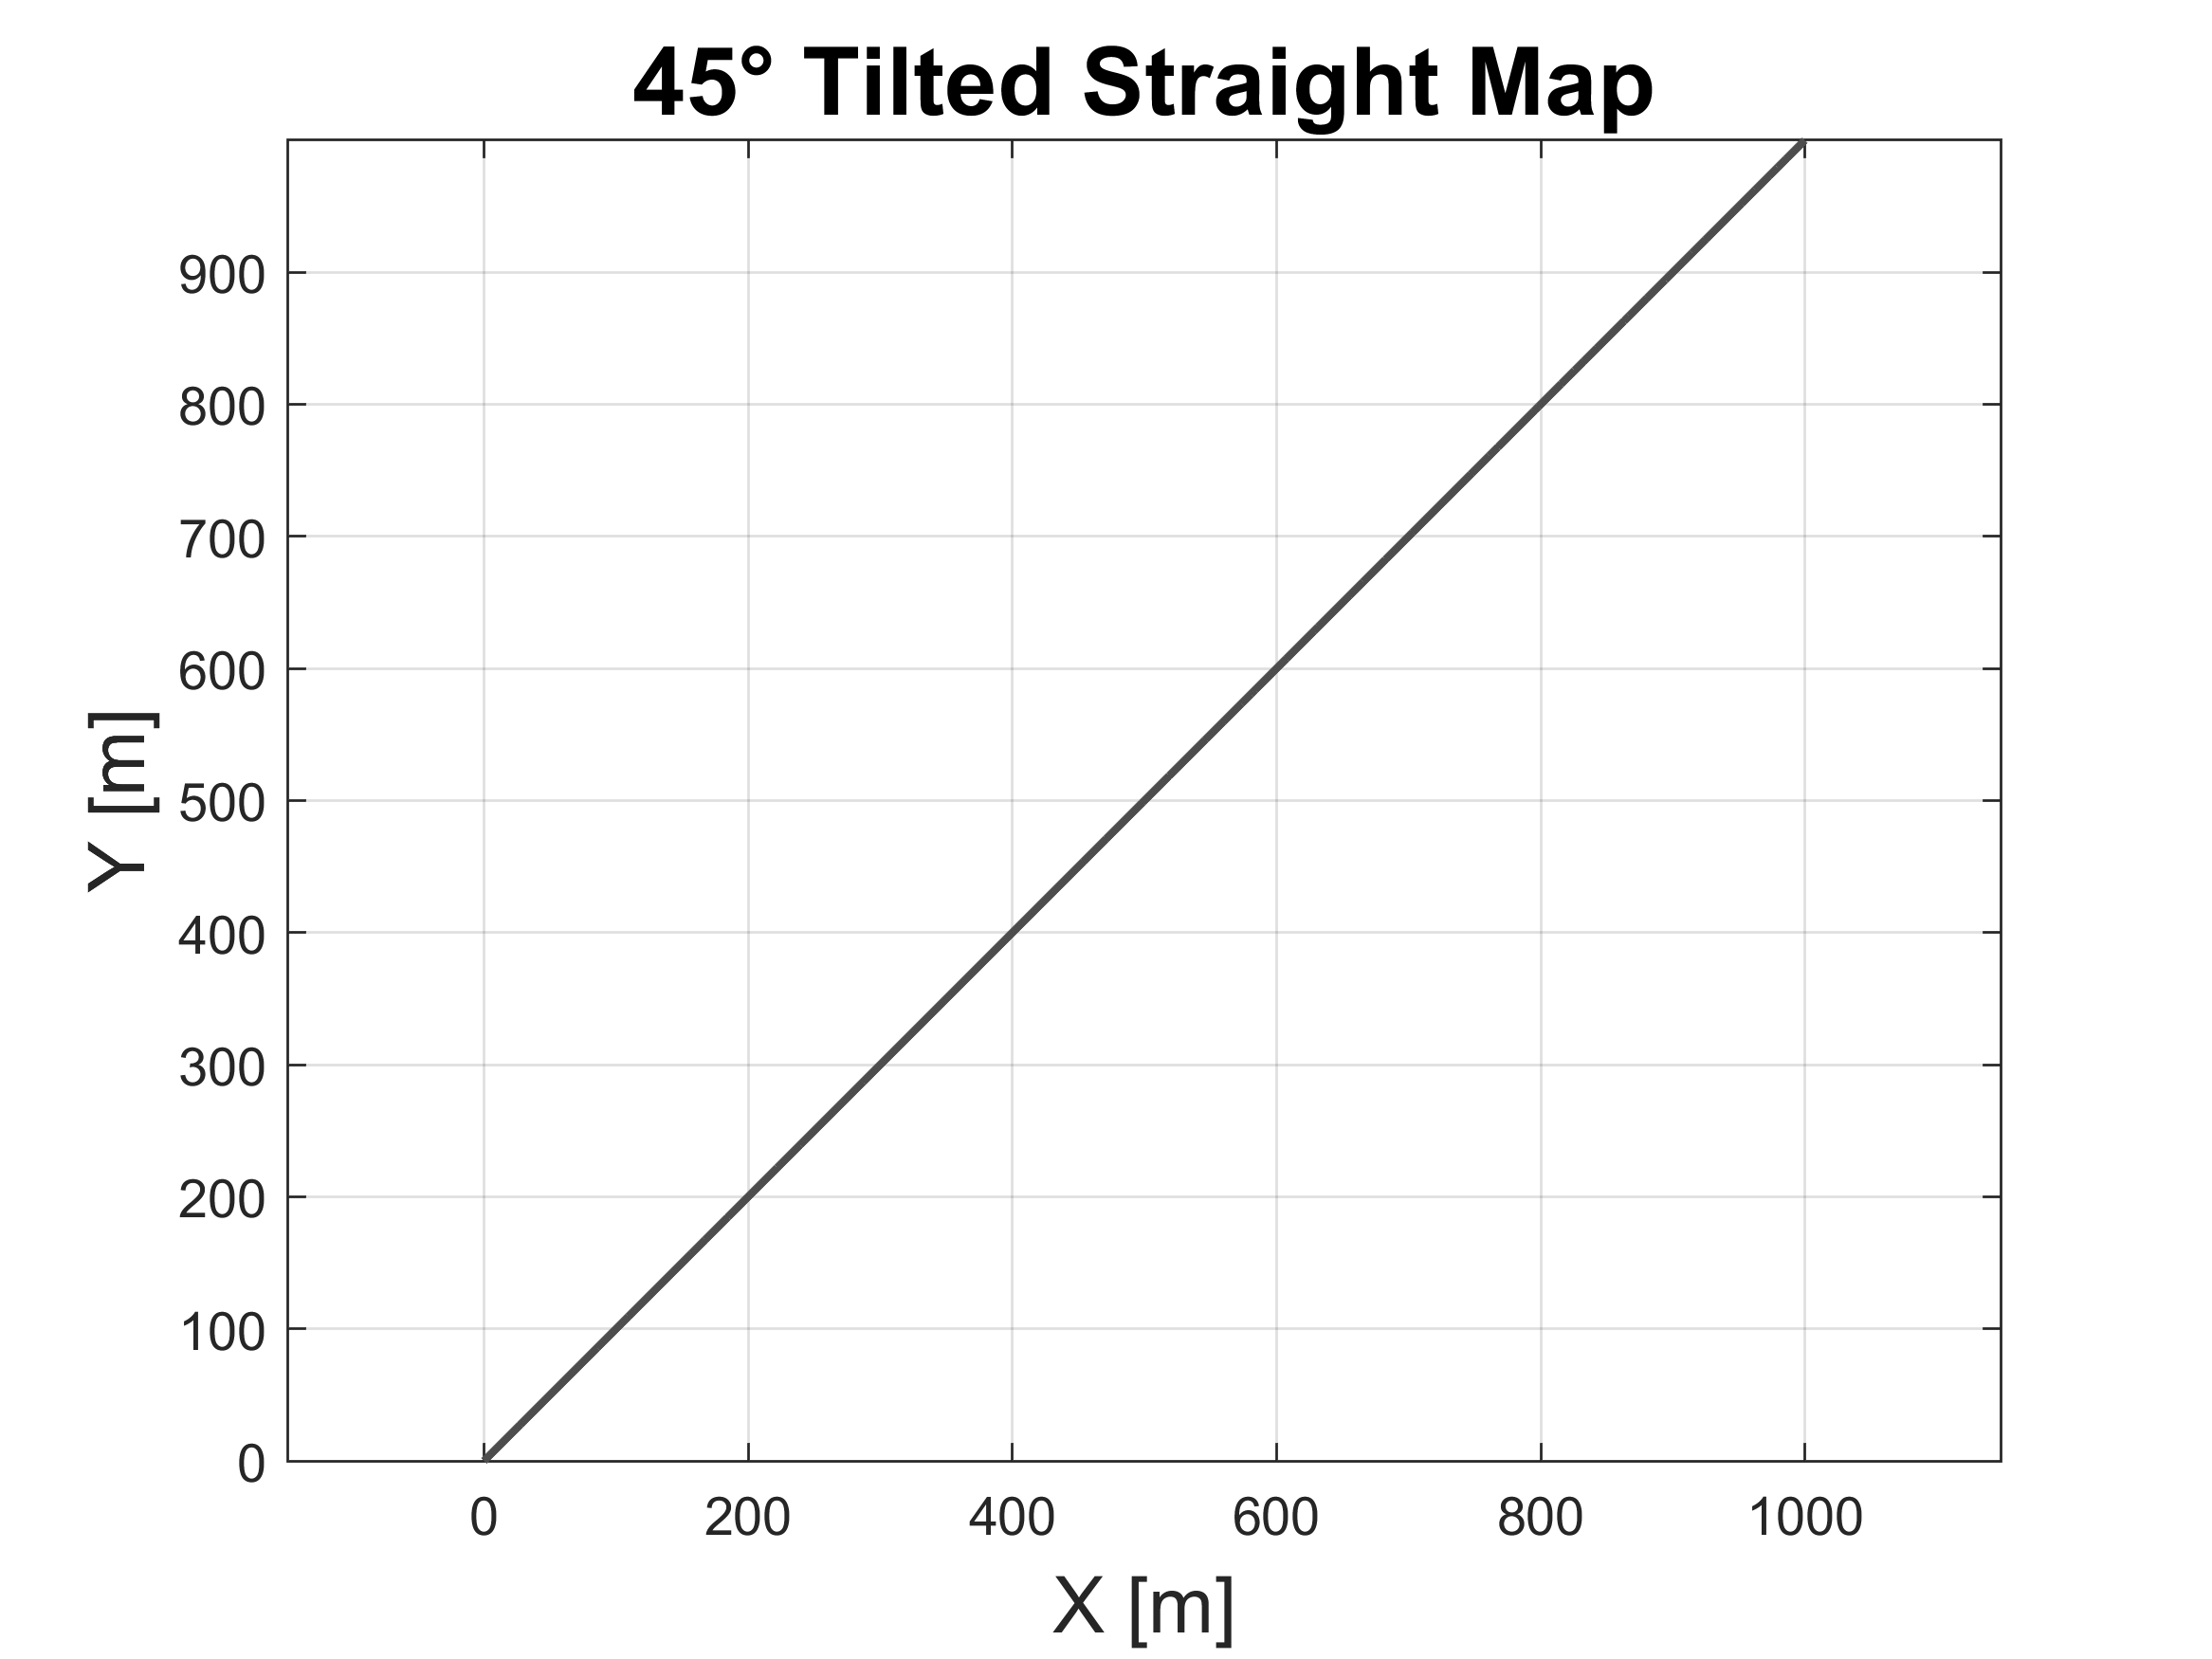
\includegraphics[width=0.7\textwidth]{Figures/Tilted45Map.png}
    \caption{Tilted straight 45° map}
      \label{fig:Tilted45Map}
\end{figure}
\pagebreak
    \item \textbf{Tilted straight line - 135°}: this is a simple scenario consisting of a straight line starting from $(0,0)$ up to $(-1000,1000)$, with an orientation of 135°. We selected a speed of 100 km/h for this scenario;
     \begin{figure}[H]
    \centering
    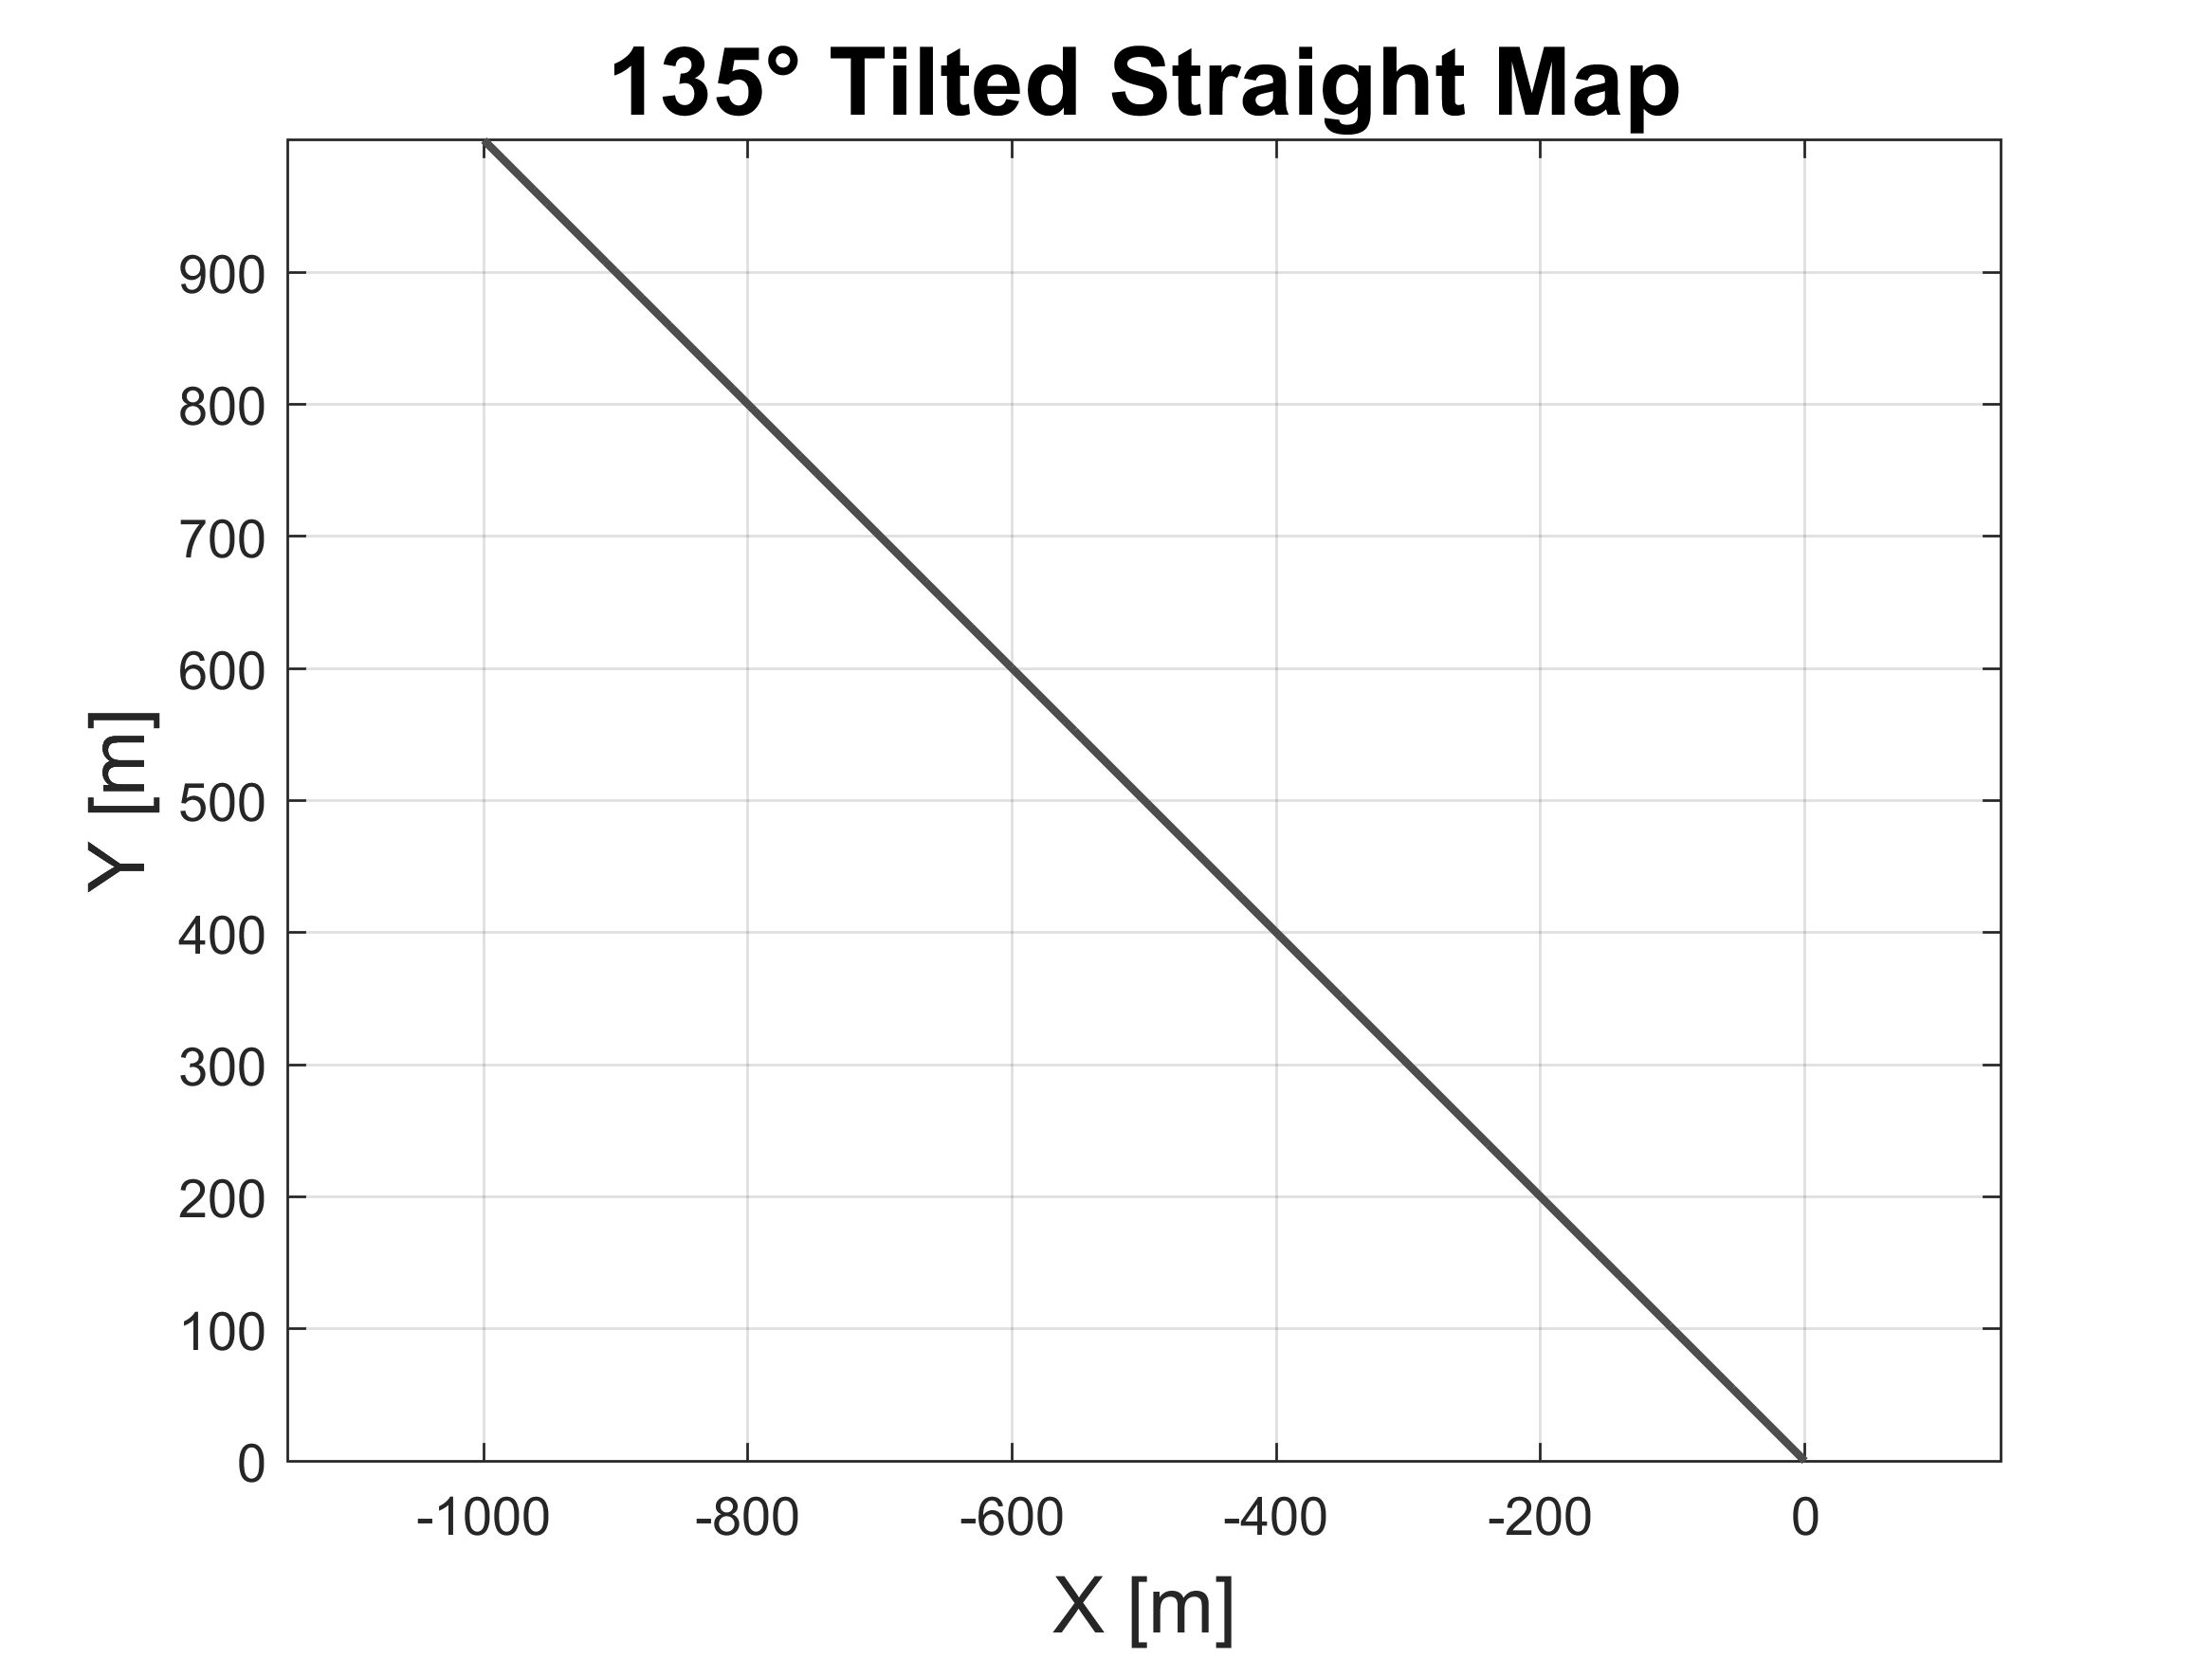
\includegraphics[width=0.7\textwidth]{Figures/Tilted135Map.png}
    \caption{Tilted straight 135° map}
      \label{fig:Tilted135Map}
\end{figure}
\vspace{1cm}
    \item \textbf{100m radius Curve}: this scenario consist of a road with constant curvature with 100 $m$ radius. We repeated this scenario twice with speeds respectively of 10 km/h and 100 km/h;
     \begin{figure}[H]
    \centering
    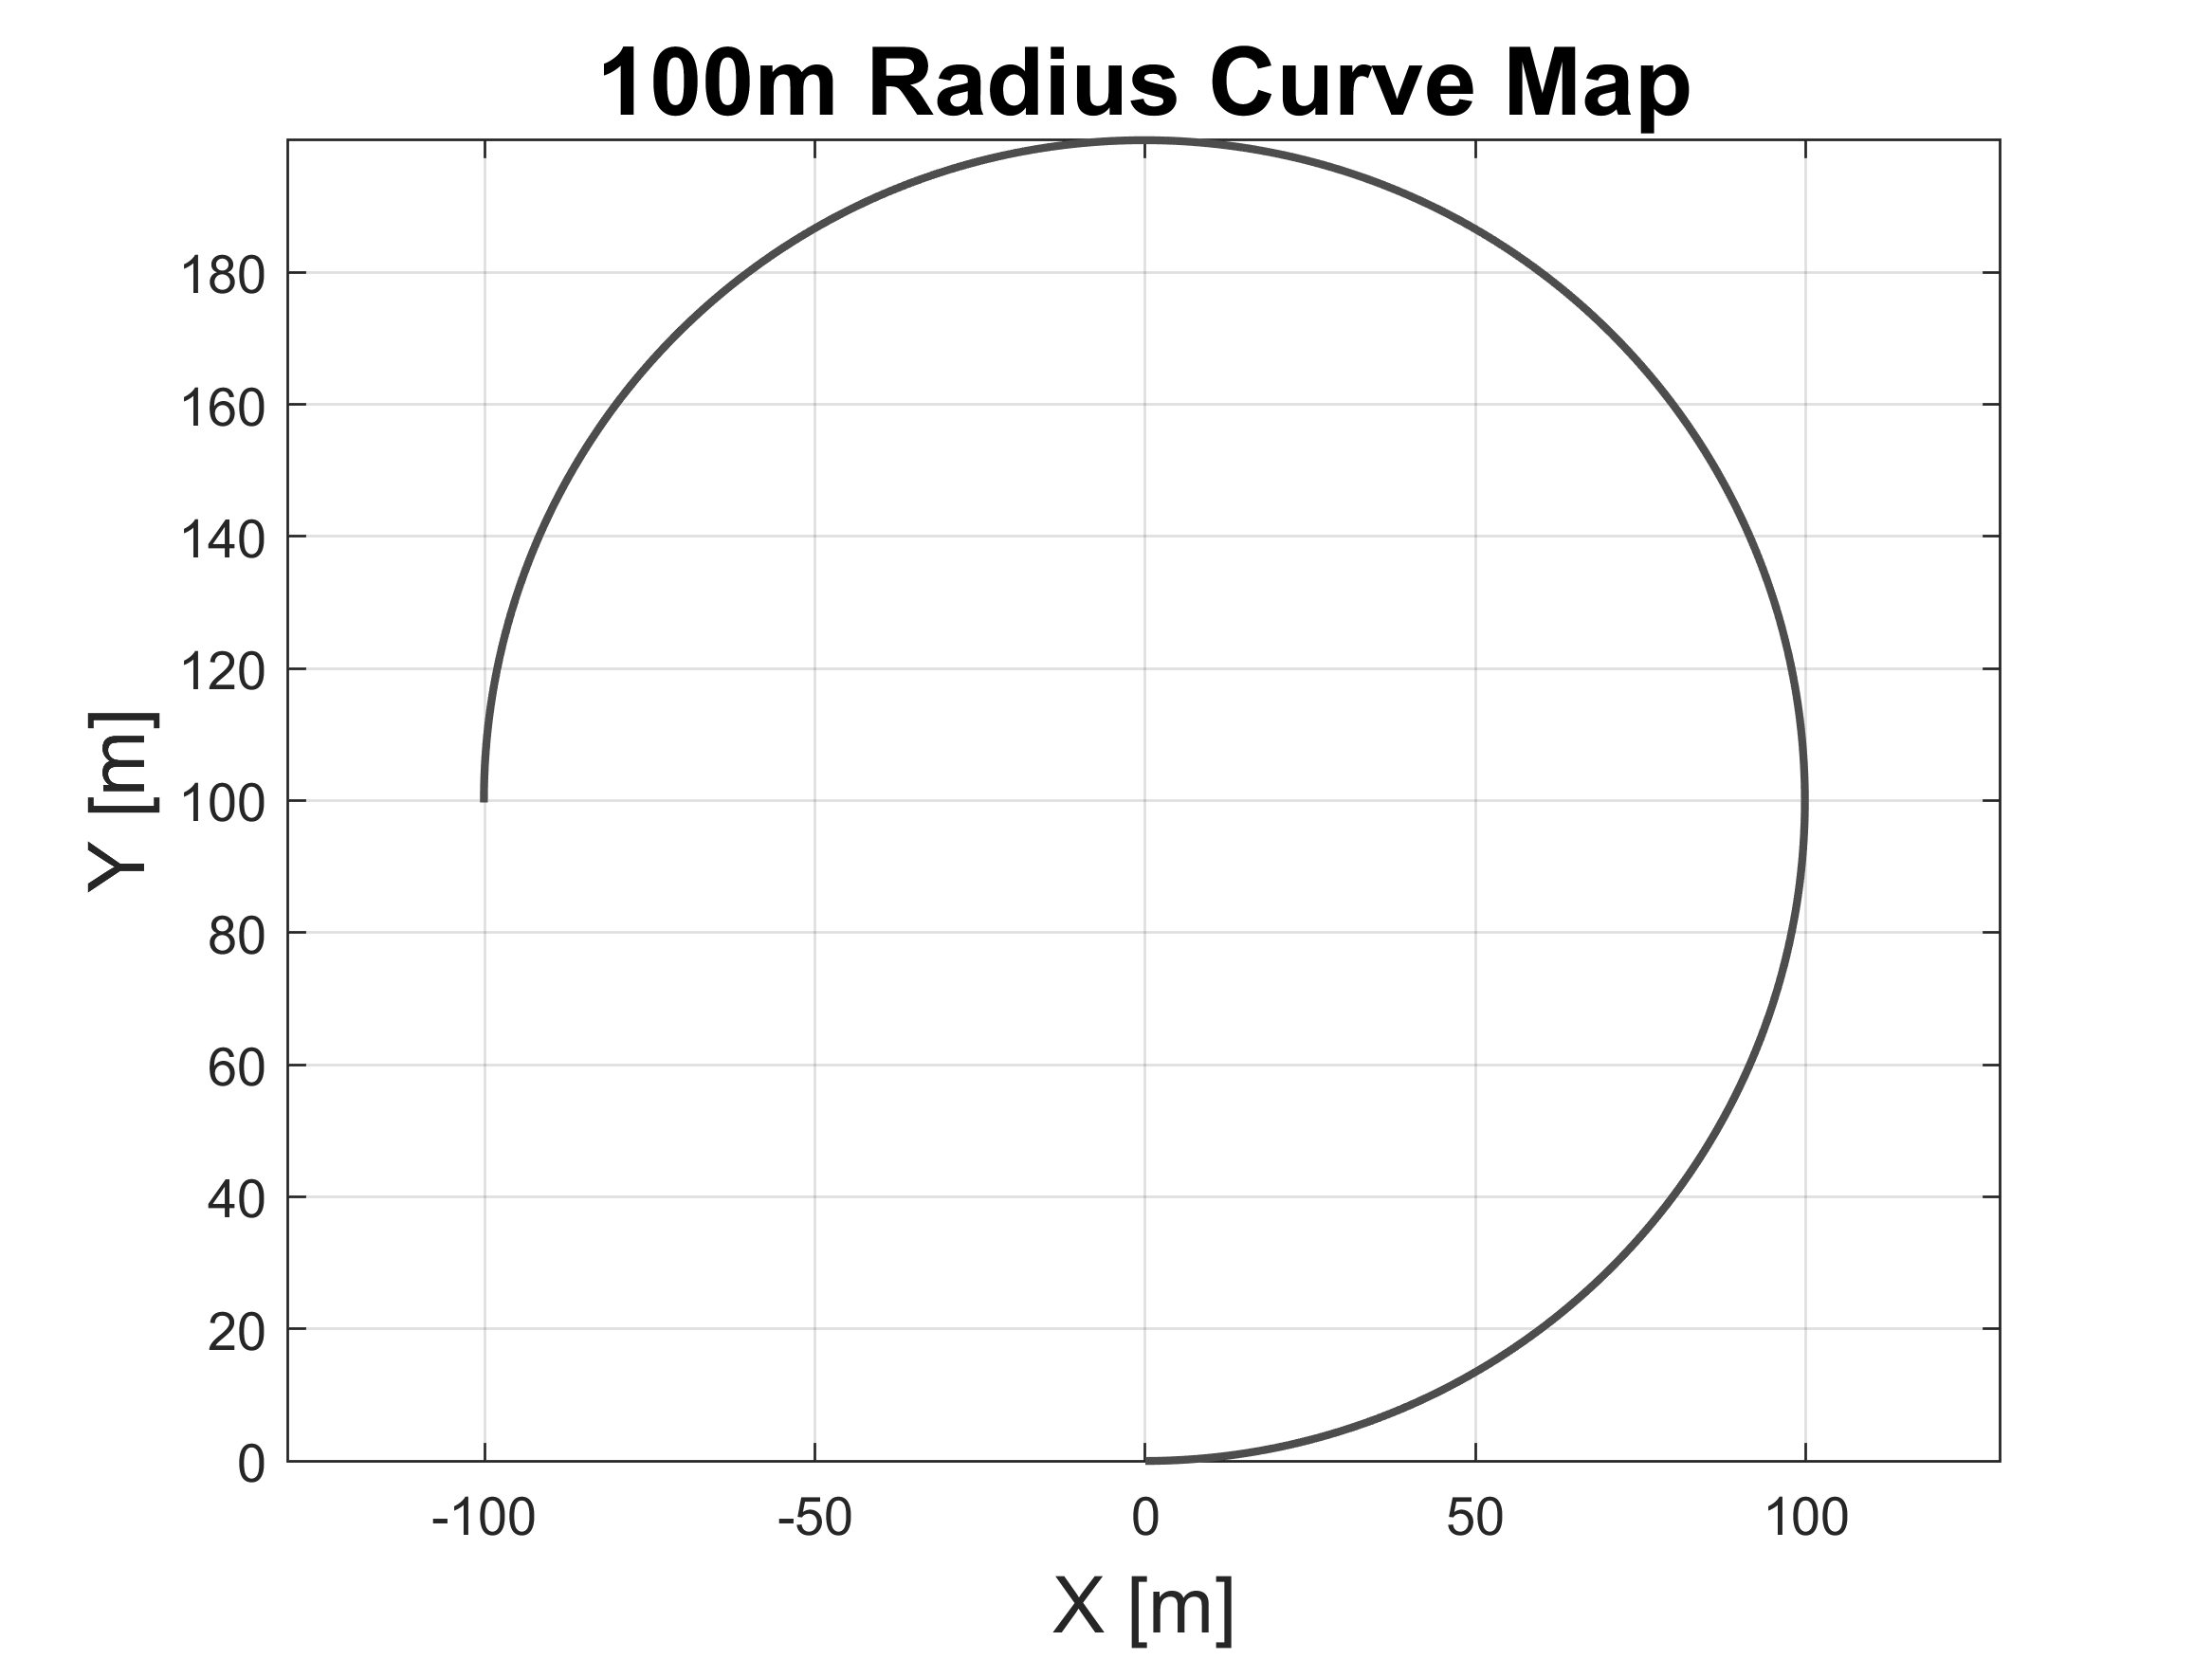
\includegraphics[width=0.7\textwidth]{Figures/ShortCurveMap.png}
    \caption{100m radius Curve Map}
      \label{fig:100mCurveMap}
\end{figure}
\pagebreak
    \item \textbf{1000m radius Curve}: this scenario consist of a road with constant curvature with 1000 $m$ radius. We repeated this scenario twice with speeds respectively of 20 km/h and 100 km/h;
     \begin{figure}[H]
    \centering
    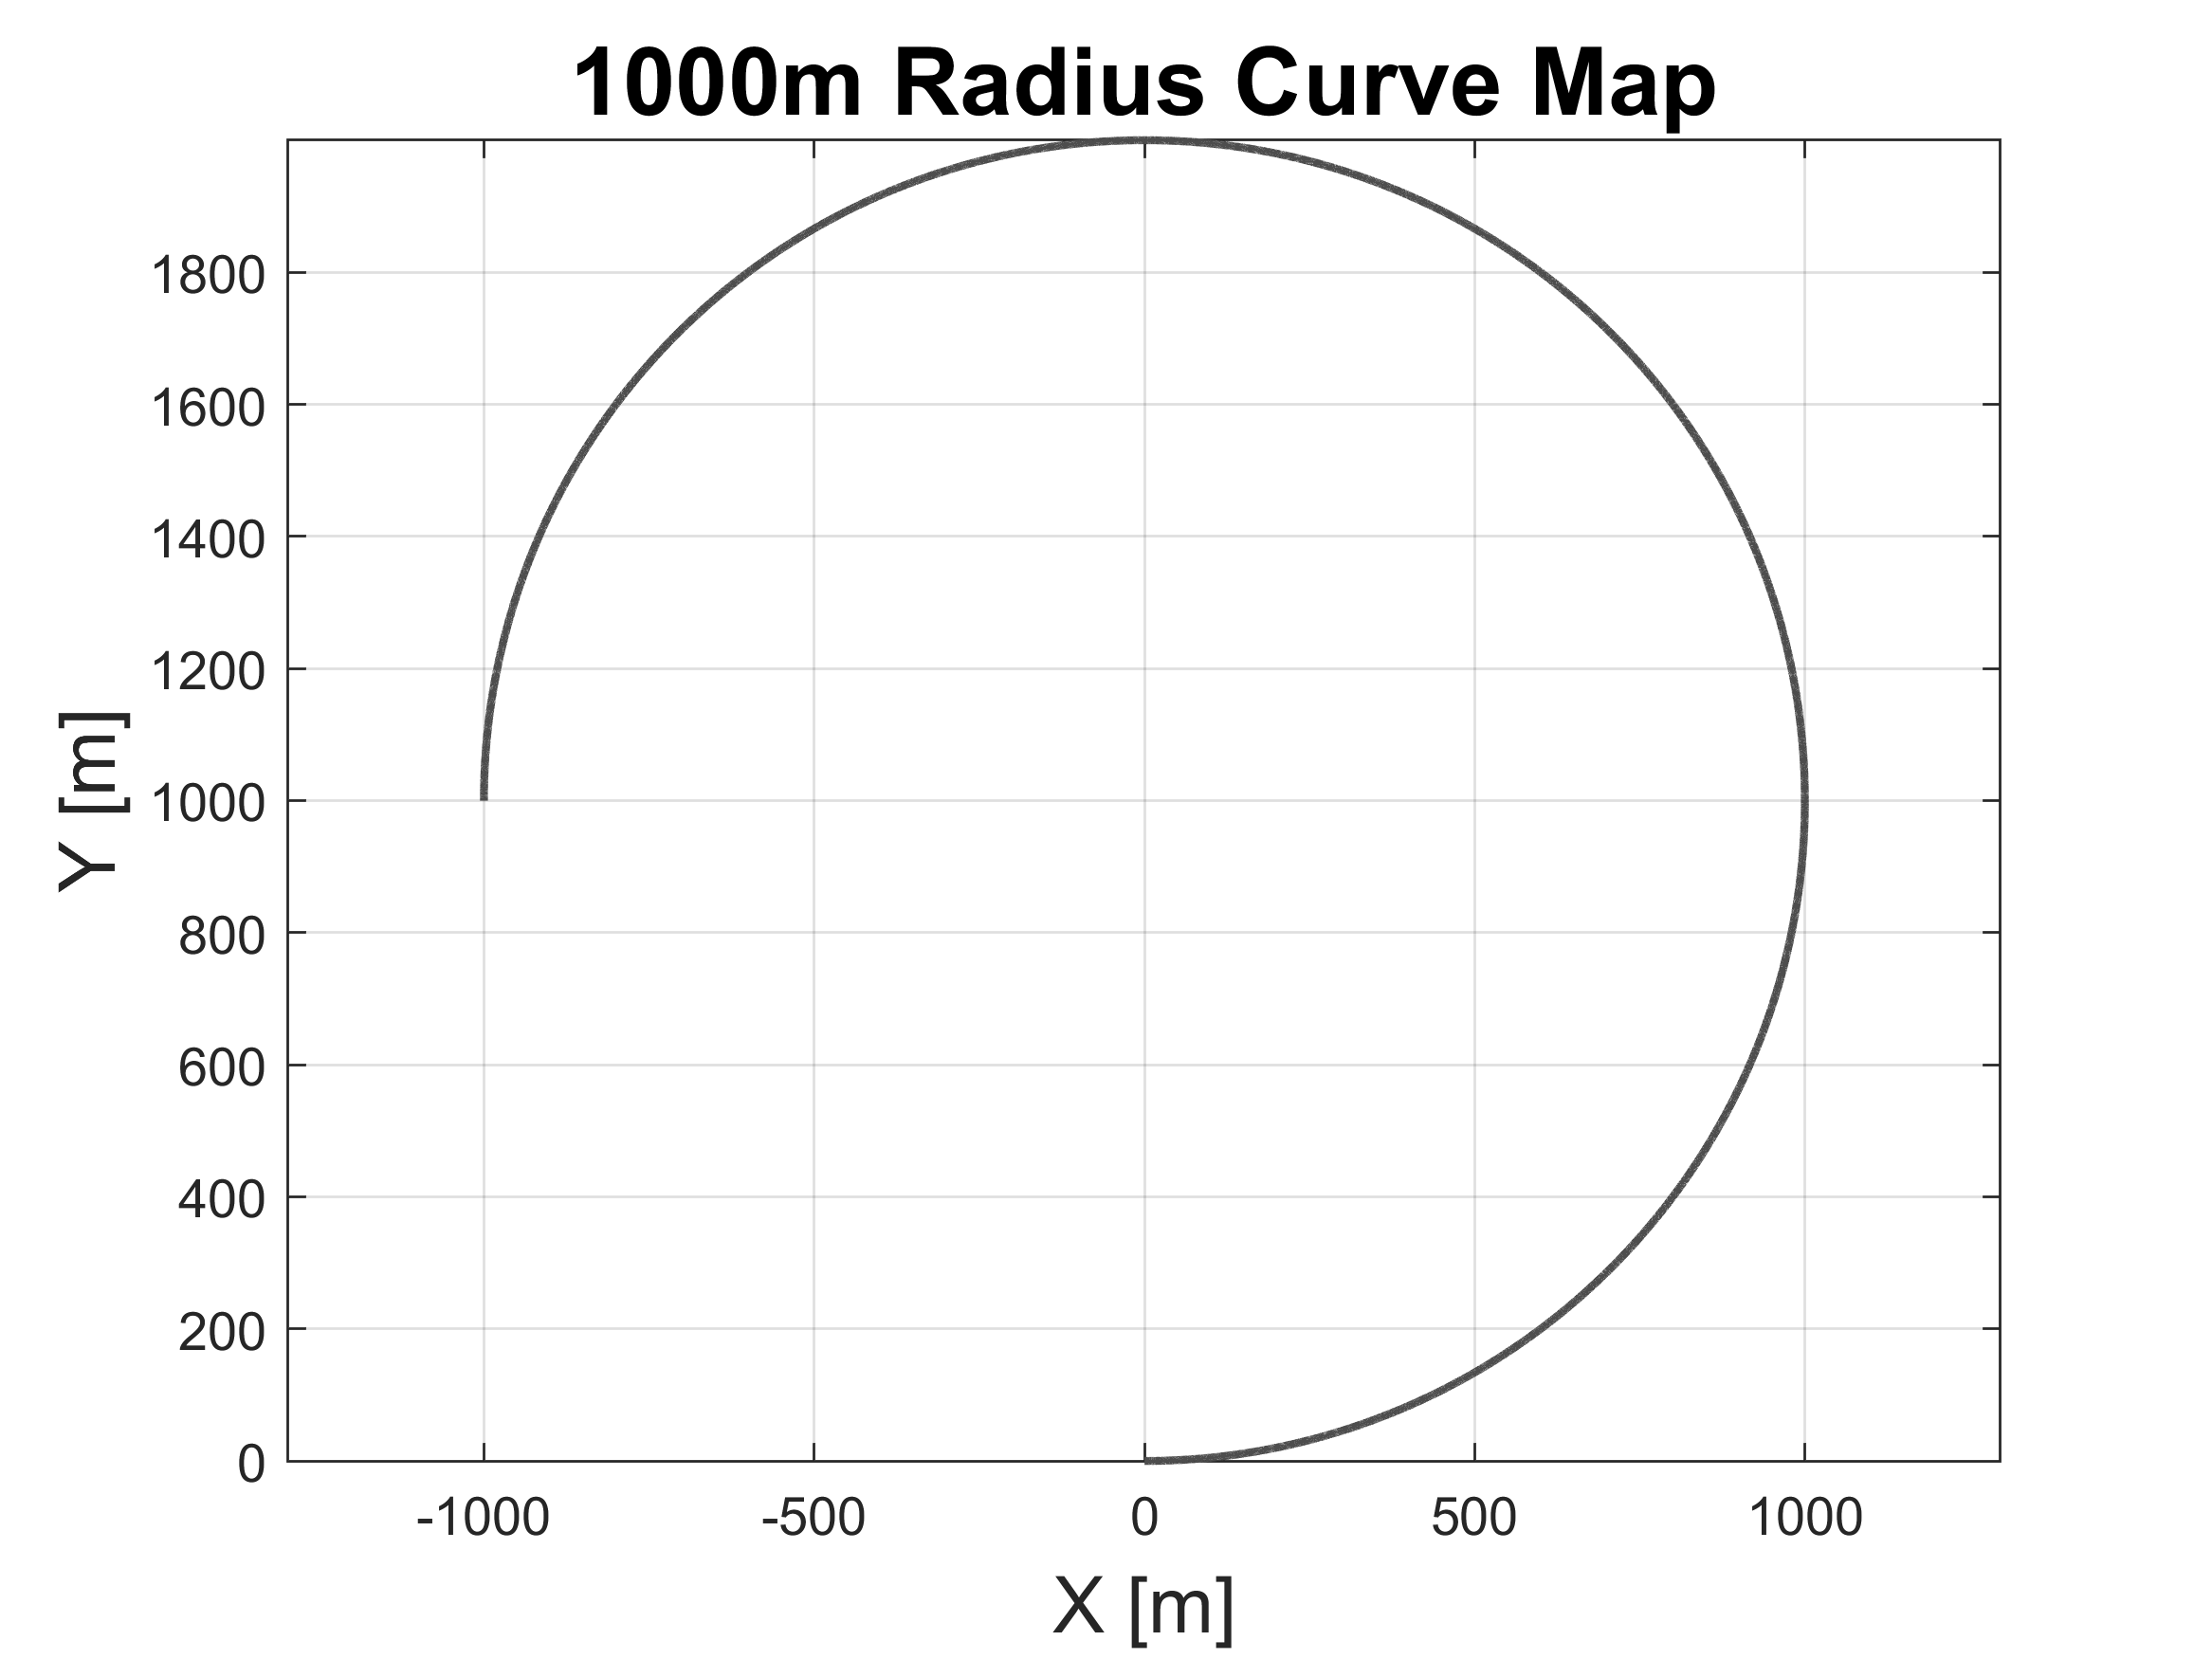
\includegraphics[width=0.7\textwidth]{Figures/LongCurveMap.png}
    \caption{1000m radius Curve Map}
      \label{fig:1000mCurveMap}
\end{figure}
\vspace{1cm}
    \item \textbf{Puglia}: this scenario is taken from a city road and it is straight for the most part with some smooth corners. In this test we try to follow the path with a speed of 40 km/h;
     \begin{figure}[H]
    \centering
    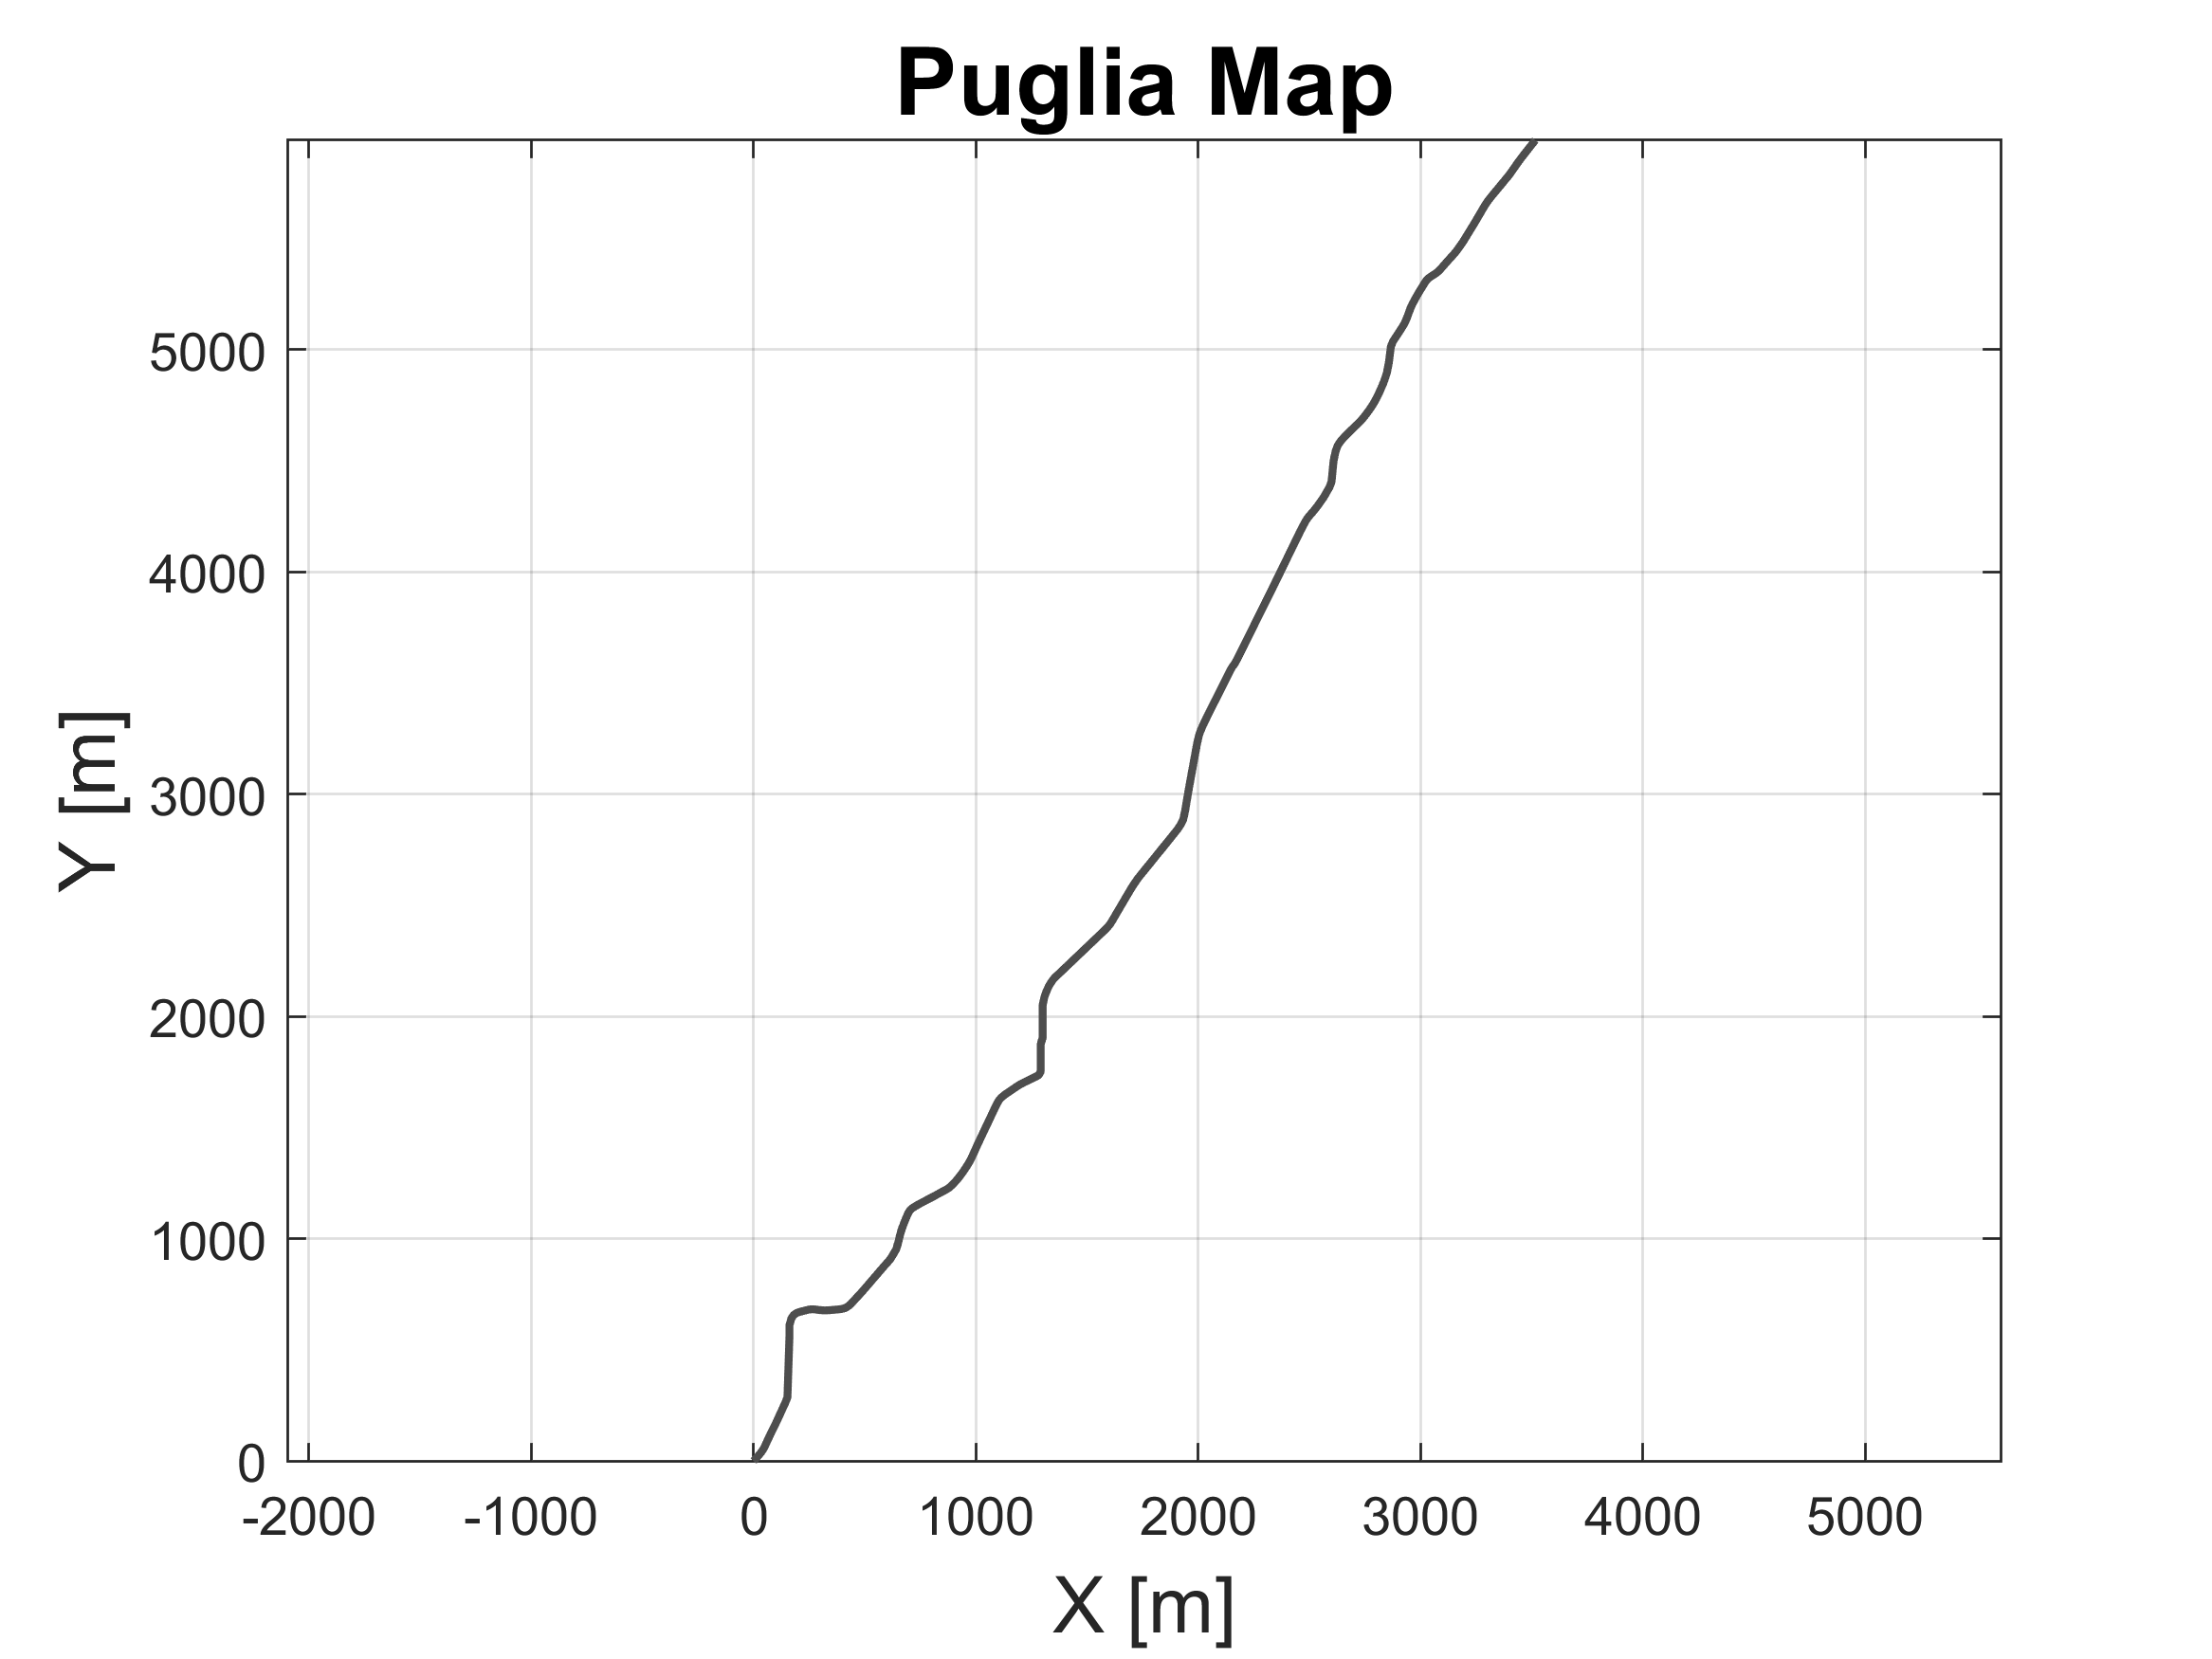
\includegraphics[width=0.7\textwidth]{Figures/PugliaMap.png}
    \caption{Puglia Map}
      \label{fig:PugliaMap}
\end{figure}
\pagebreak
    \item \textbf{Switzerland}: this is the slowest scenario considered, with lots of corners one after another. We try to follow this scenario with 15 km/h speed;
     \begin{figure}[H]
    \centering
    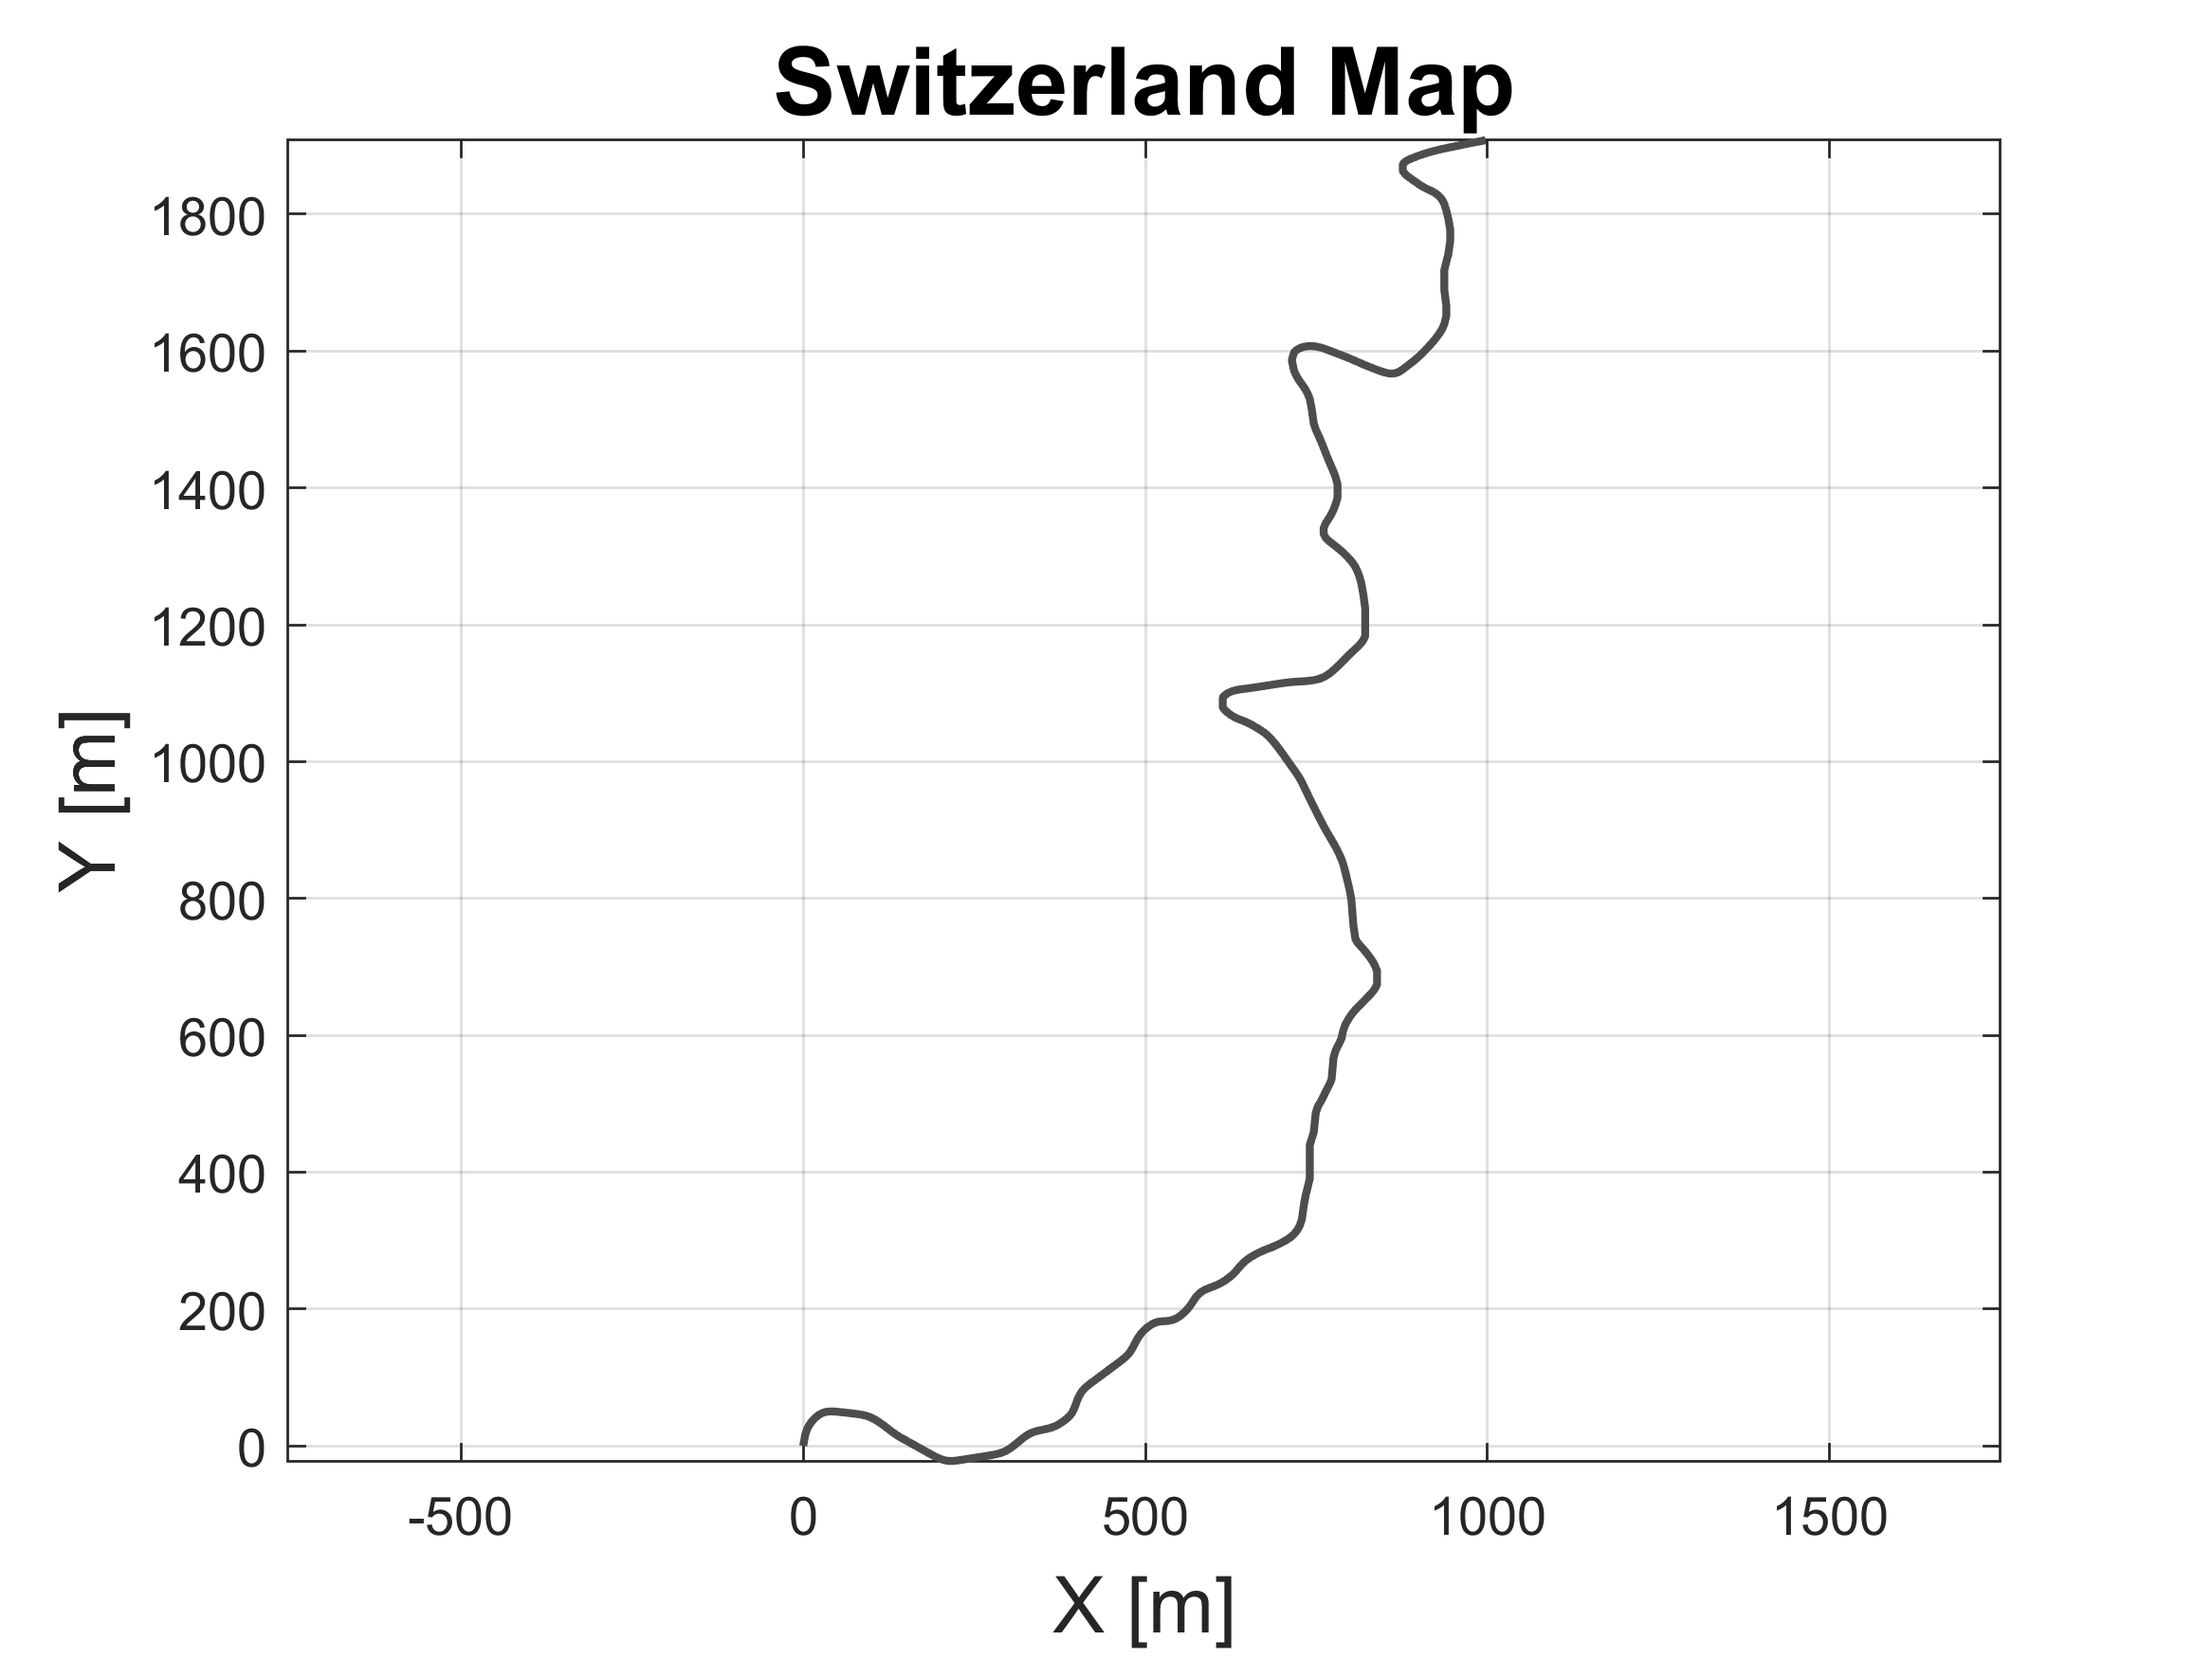
\includegraphics[width=0.7\textwidth]{Figures/SwitzerlandMap.png}
    \caption{Switzerland Map}
      \label{fig:SwitzerlandMap}
\end{figure}
\vspace{1cm}
    \item \textbf{Campania}: this scenario is made up by a sequence of smooth corners. We try to follow this path with 30 km/h speed;
     \begin{figure}[H]
    \centering
    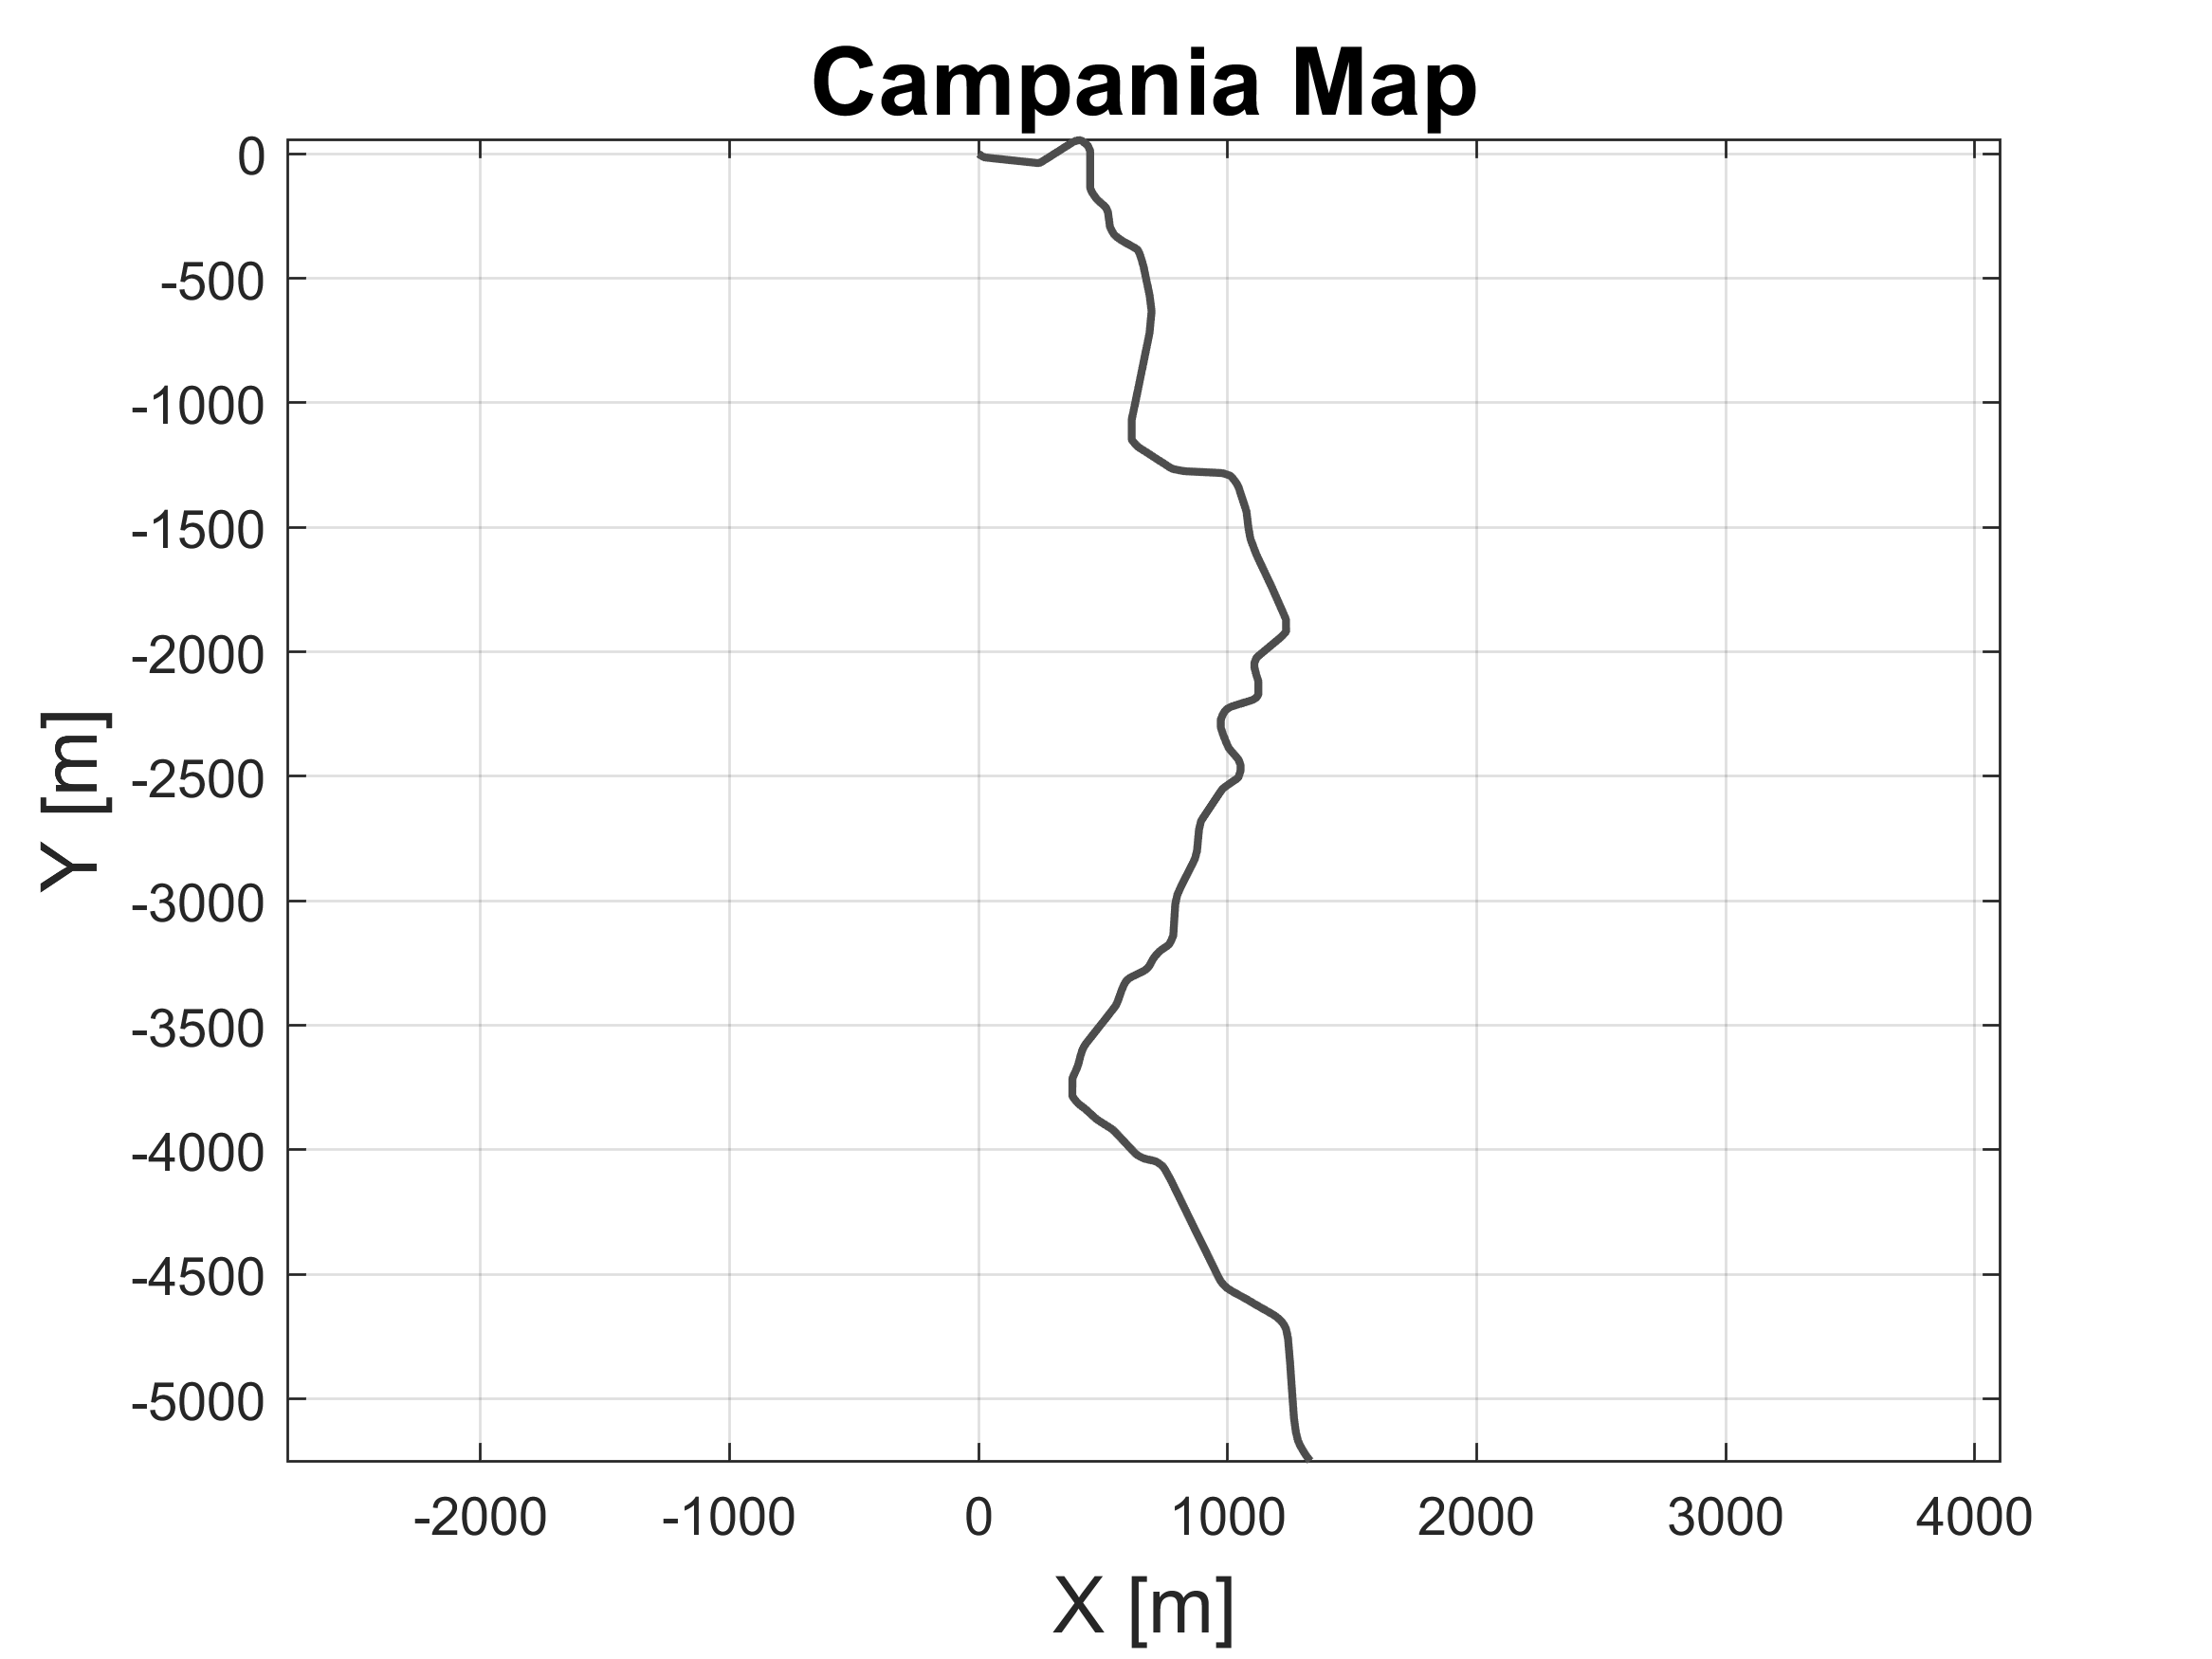
\includegraphics[width=0.7\textwidth]{Figures/CampaniaMap.png}
    \caption{Campania Map}
      \label{fig:Campania}
\end{figure}
\pagebreak
    \item \textbf{Adriatic Highway - A14}: This scenario is taken from the A14 highway which is a straight road for the most of it, with some highspeed corners. We simulate this scenario at 100 km/h;
     \begin{figure}[H]
    \centering
    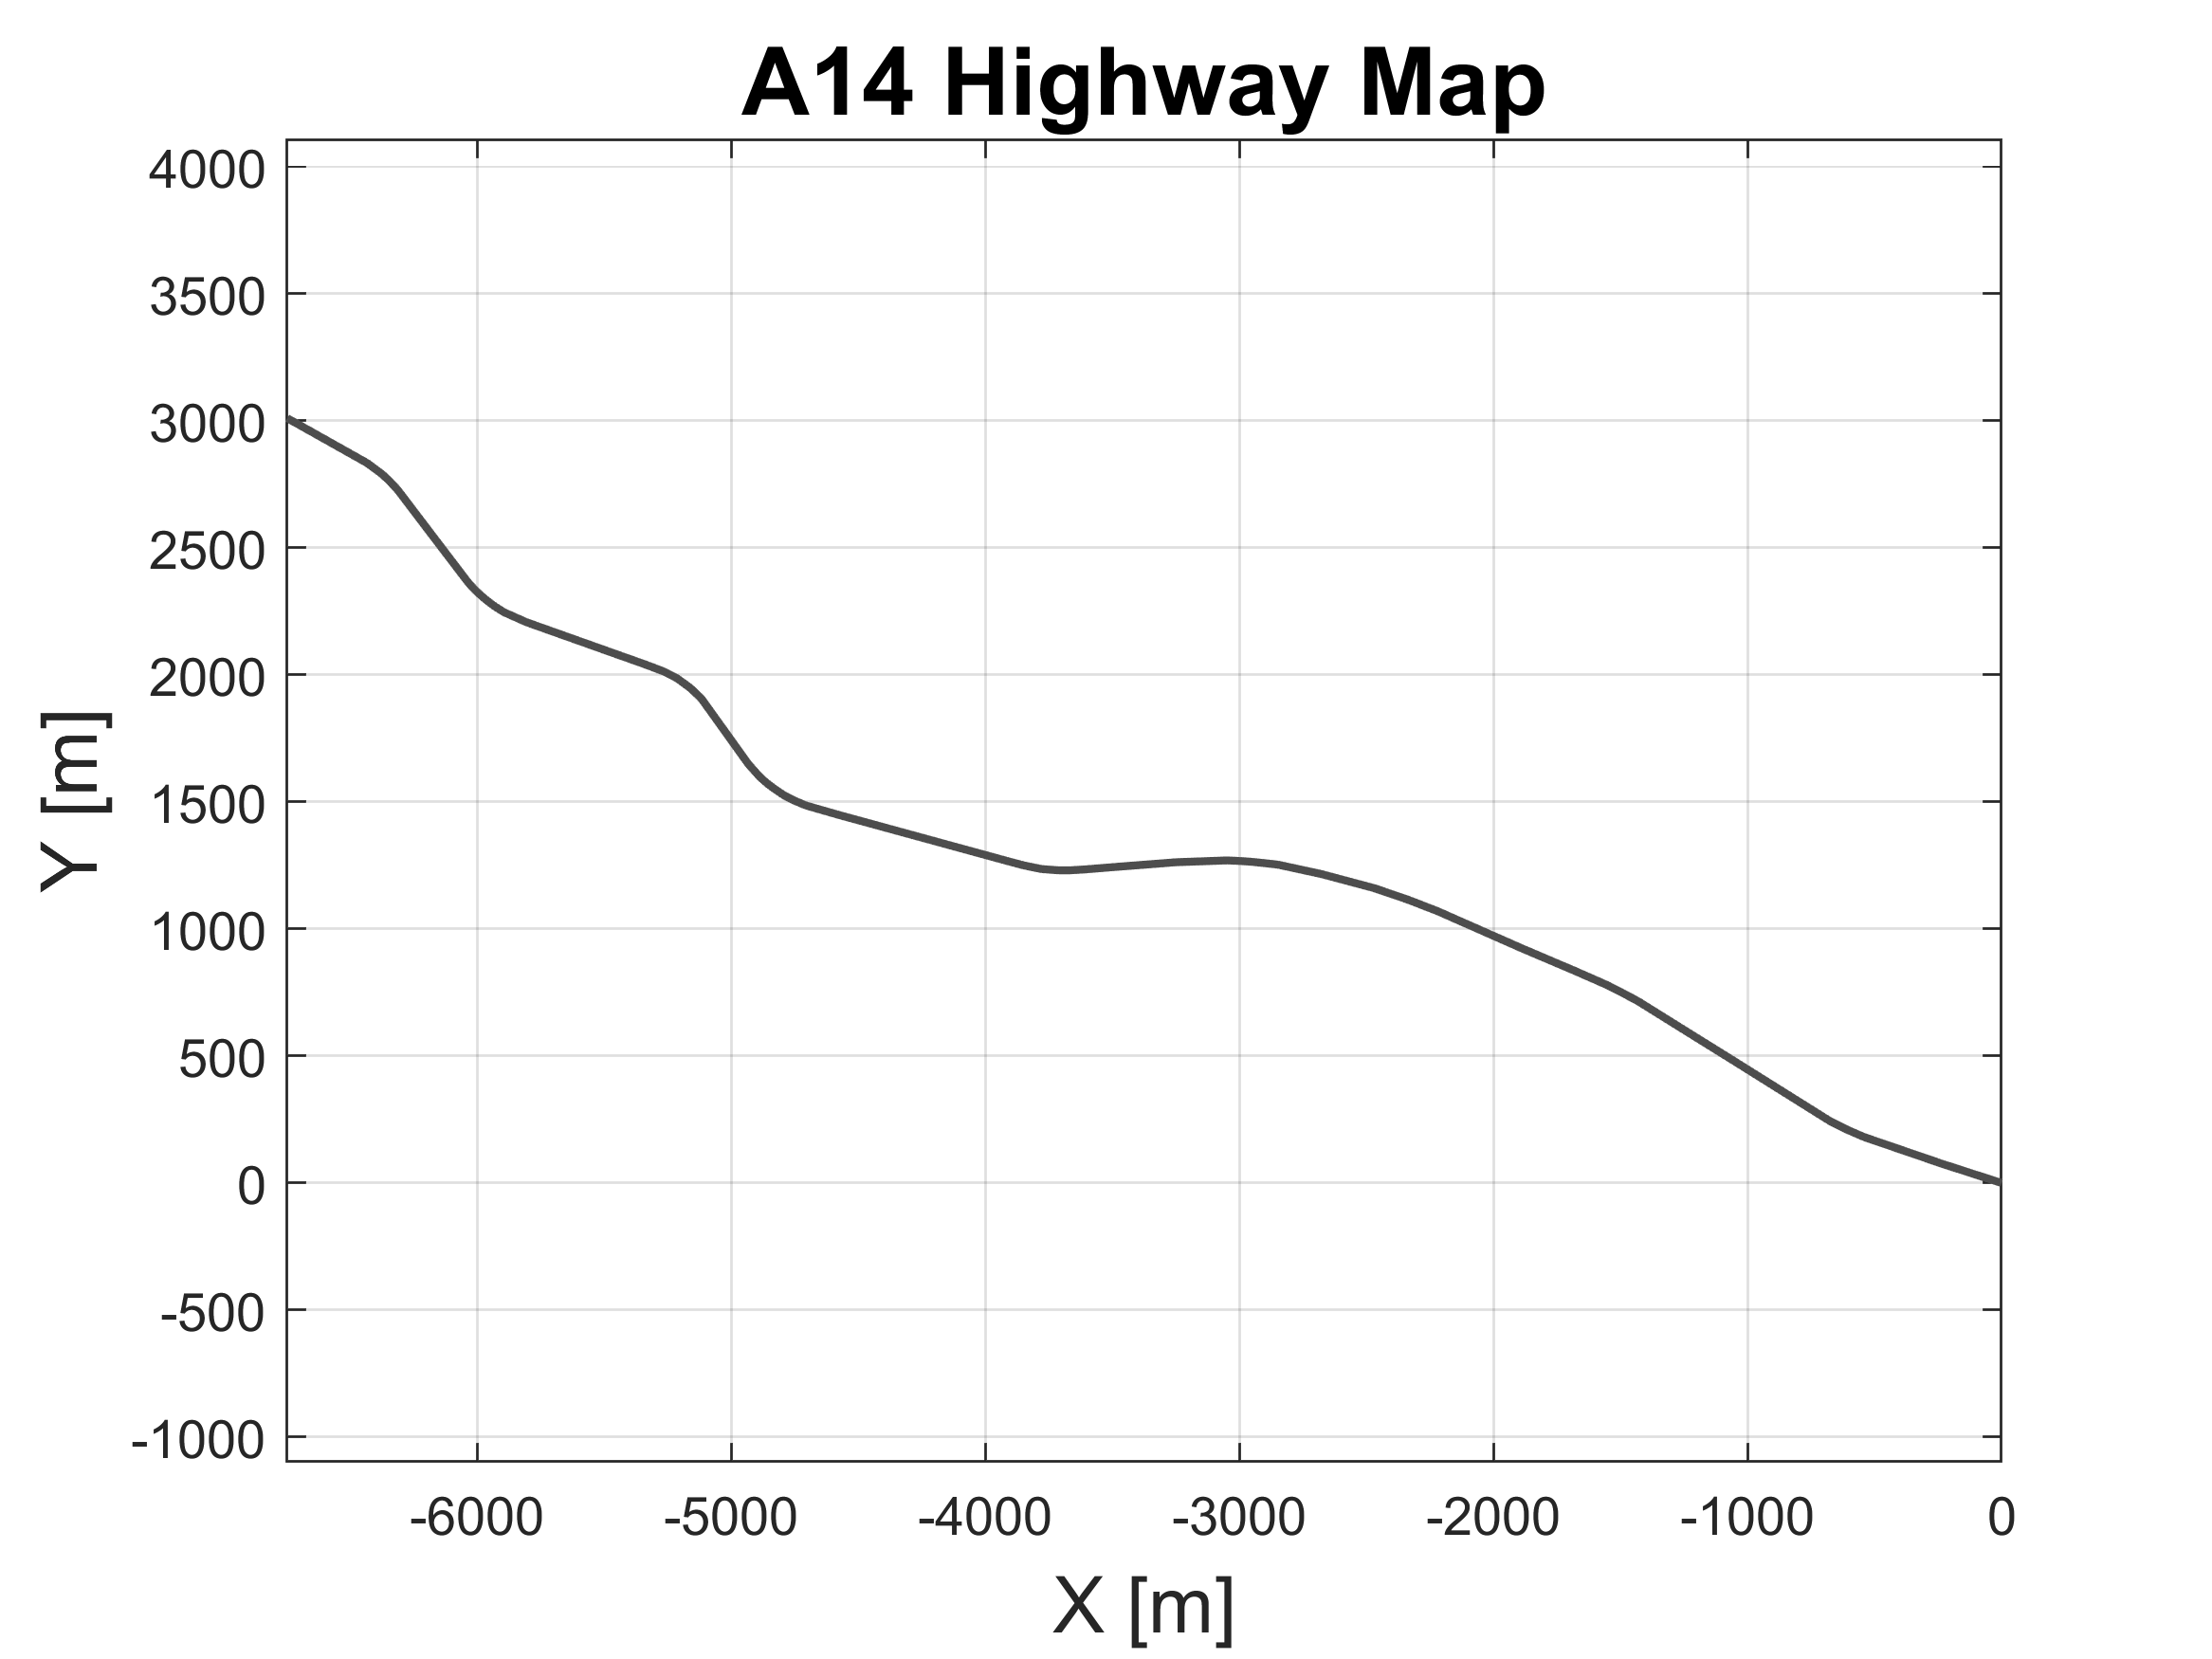
\includegraphics[width=0.7\textwidth]{Figures/A14Map.png}
    \caption{Adriatic Highway - A14 Map}
      \label{fig:A14Map}
\end{figure}
\vspace{1cm}
    \item \textbf{Indianapolis Speedway}: This scenario is taken from the Indianapolis Speedway. We simulate it at 100 km/h.
    \begin{figure}[H]
    \centering
    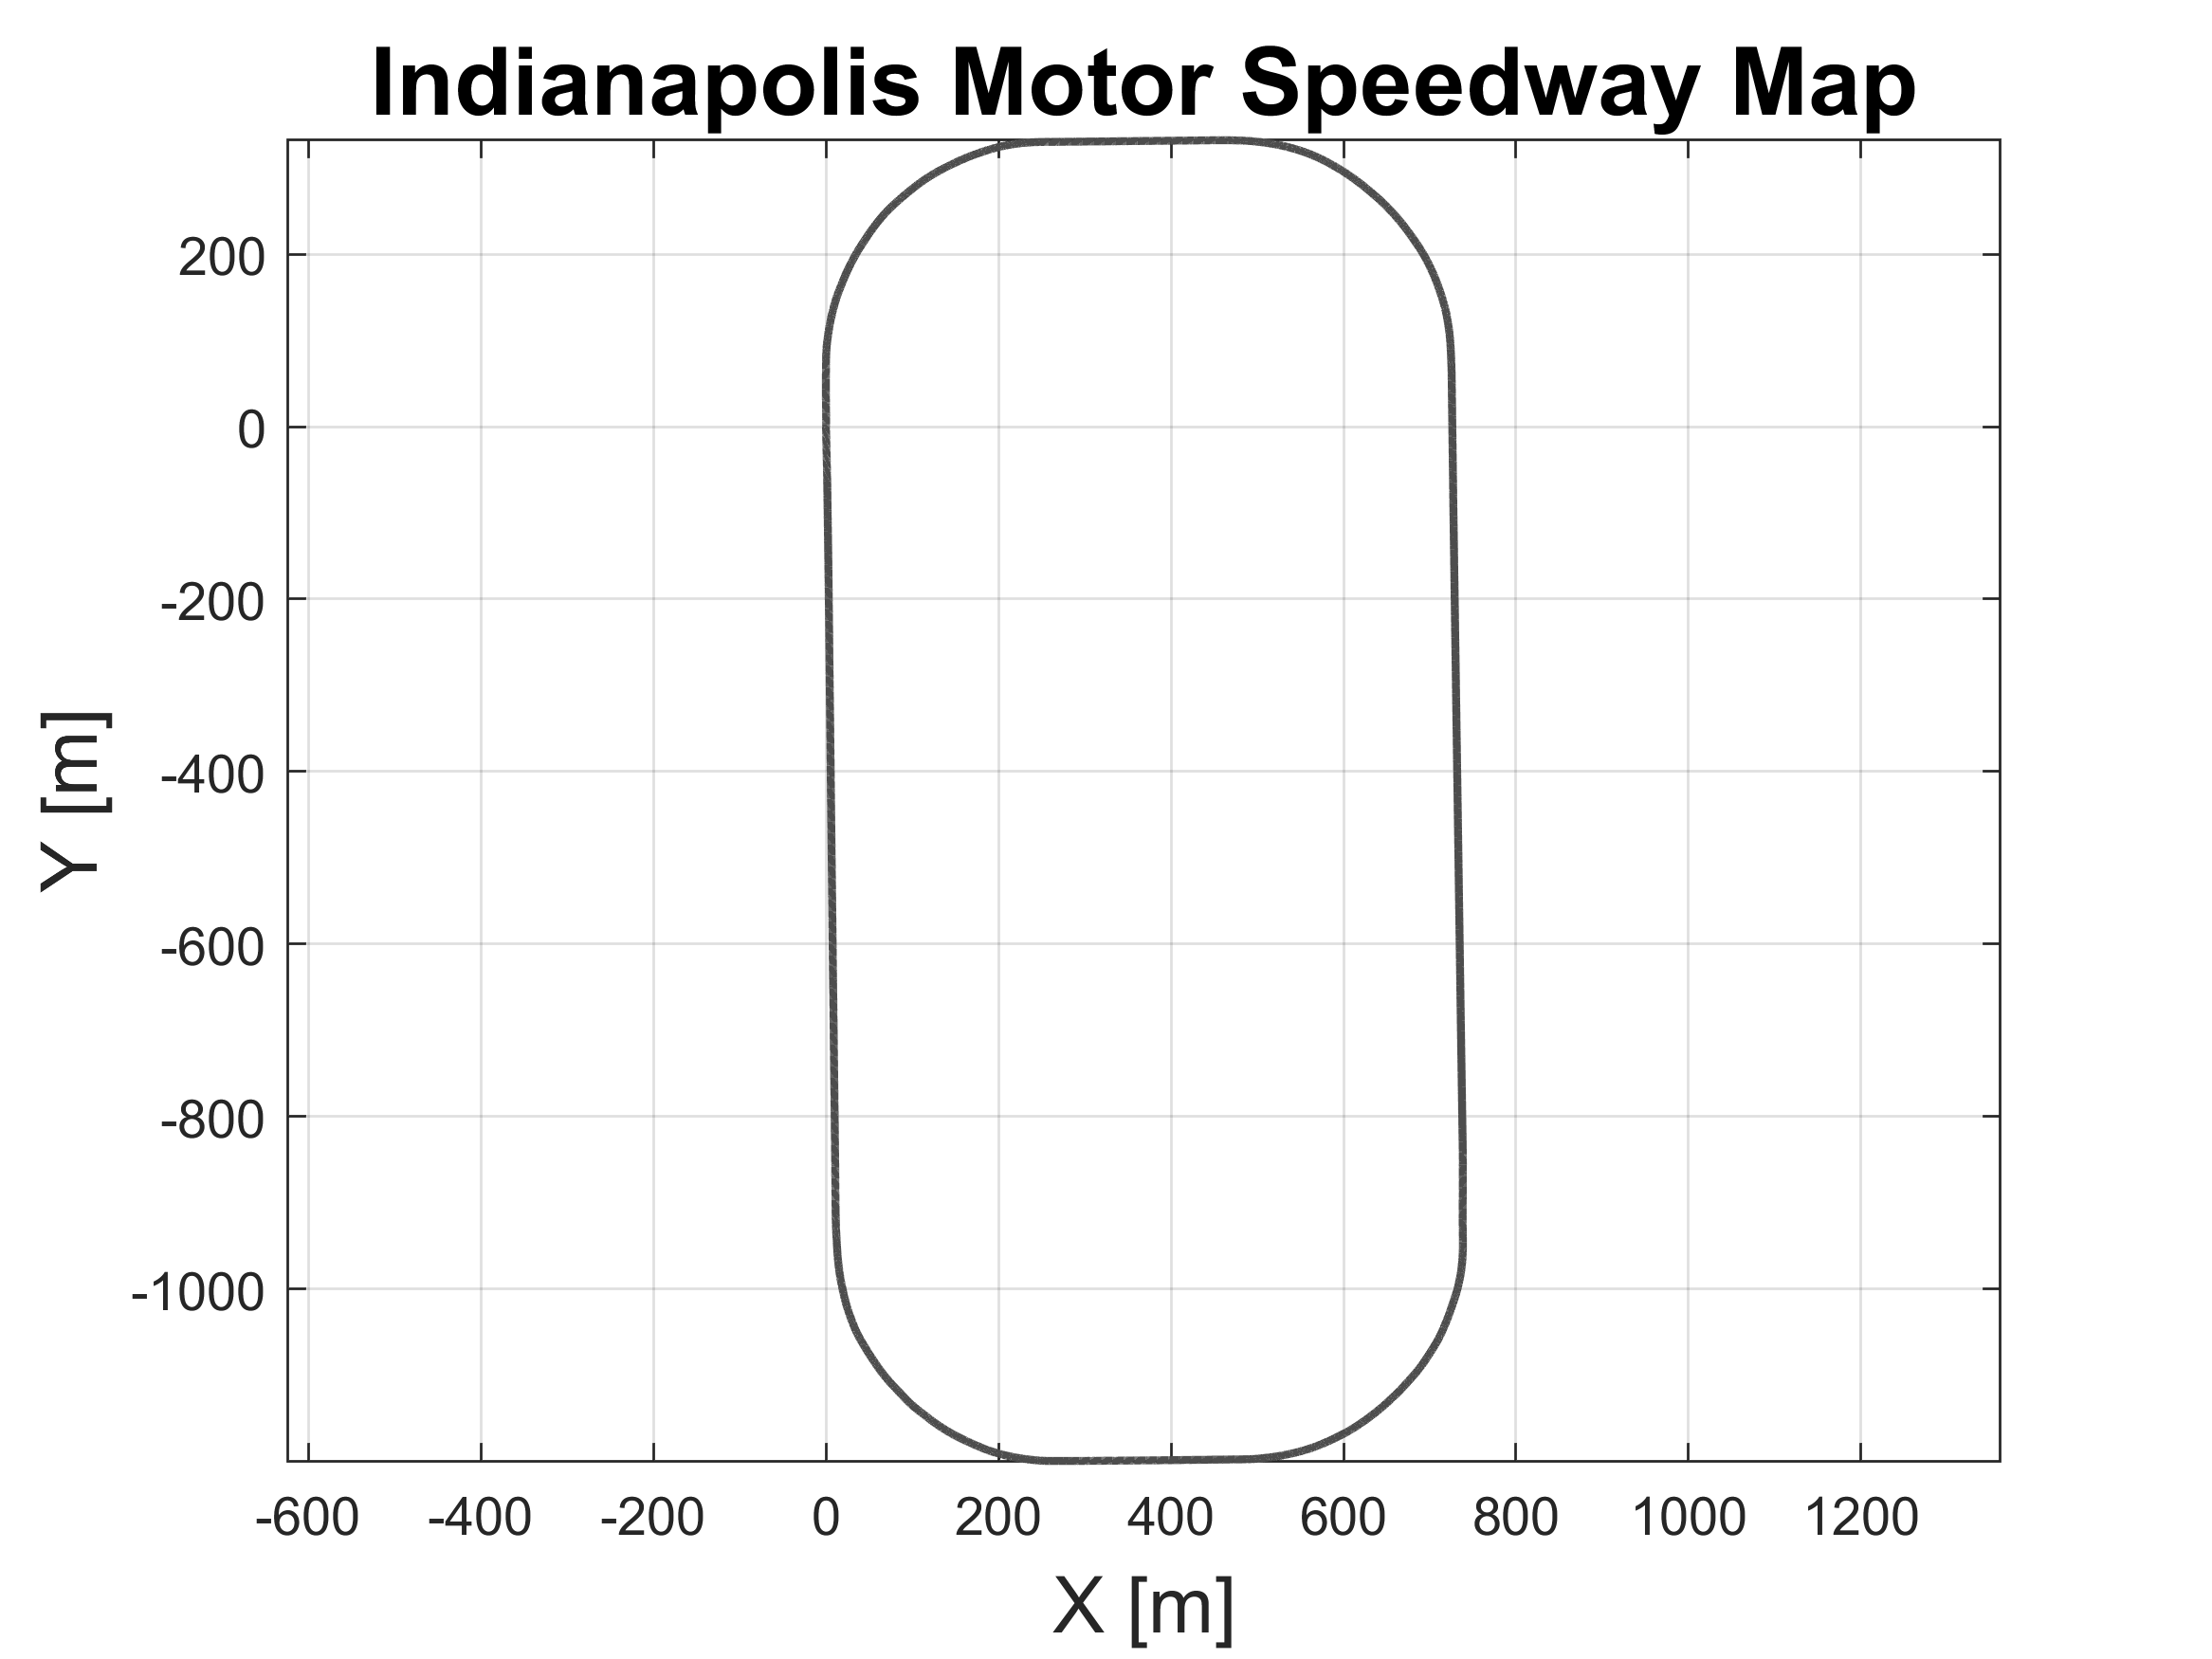
\includegraphics[width=0.7\textwidth]{Figures/IndianapolisMap.png}
    \caption{Indianapolis Speedway Map}
      \label{fig:Indianapolis}
\end{figure}
\end{enumerate}

\pagebreak
Details about the path-following tests performed can be found in the documents included in the repository\footnote{The ``Path\_Following-Test\_Report", the ``Path\_Following\_Test-Annex\_A" and the ``Path\_Following-Test\_Report - Failed Tests" files generated by Simulink Test are included in the /Documentation/Test Reports/ file path.}.\\
Performing the tests we have found that in simple scenarios, such as straight lines and Highway, the performances of our controller are very good, with little deviation from the reference path, while in winding scenarios, such as the \textit{Switzerland} one, we found out that the vehicle is not able to keep its position inside the road boundaries in all the corners.
Figures \ref{subfig:A14} and \ref{subfig:Switzerland} show the lateral deviation found in the test performed on the Adriatic Highway A14 and the one found in Switzerland respectively. As shown below, the lateral deviation in the former never exceeds the limits imposed (described at the beginning of this section), while in the latter these limits are exceeded a few times resulting in the failure of the test.


\begin{figure}[H]
\centering

    \begin{subfigure}{.5\textwidth}
    \centering
   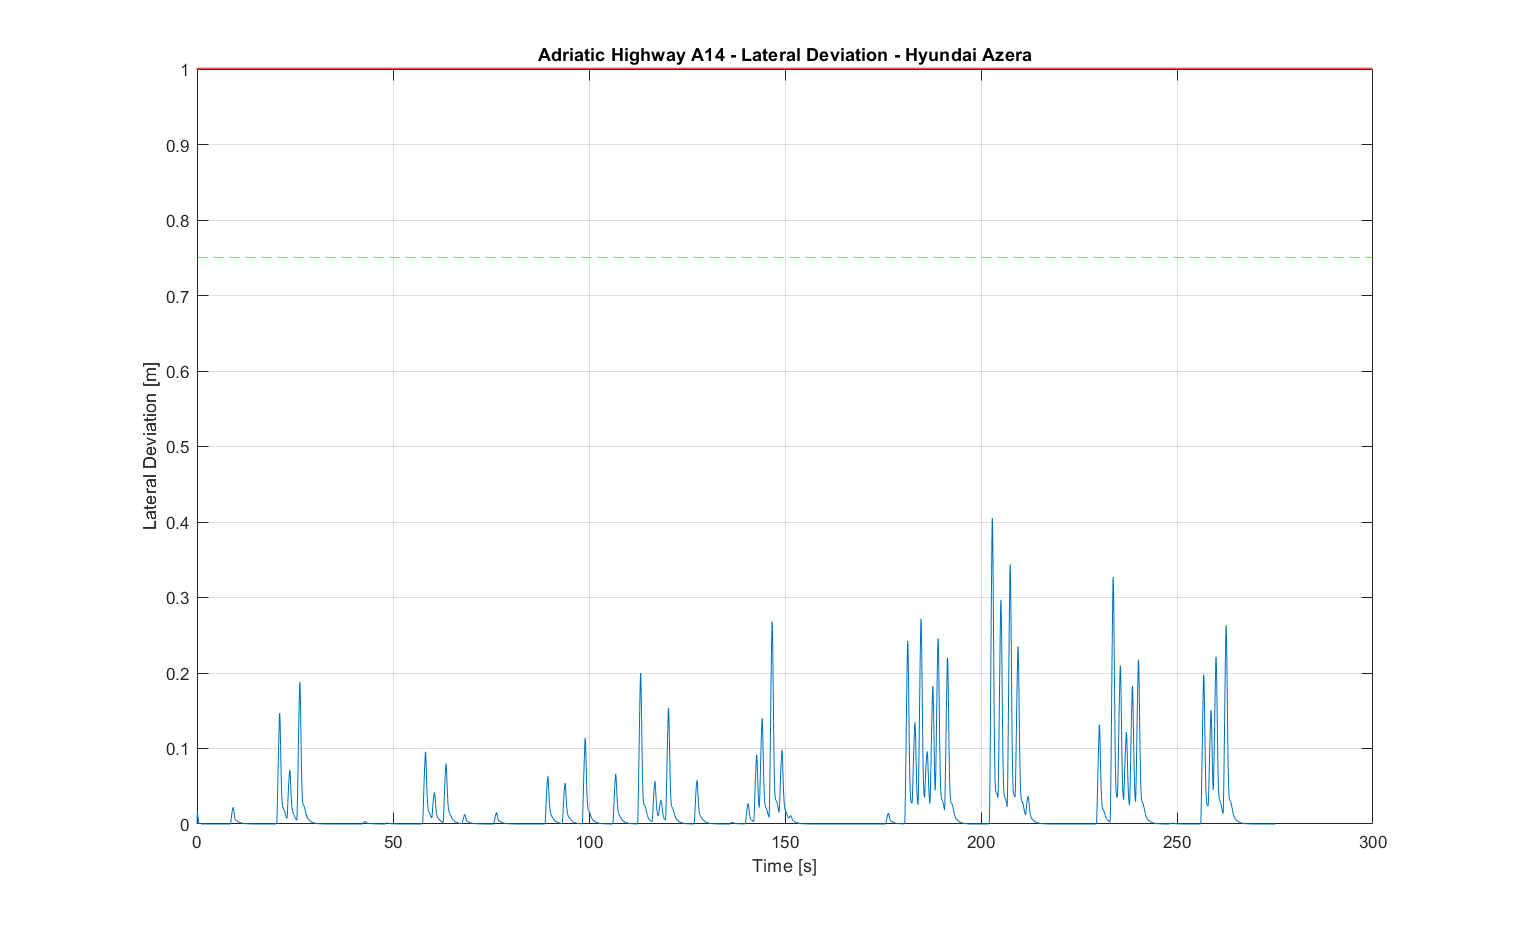
\includegraphics[width=\textwidth,keepaspectratio]{Figures/A14_lateralDev.png}
    \caption{Lateral Deviation Plot (Adriatic Highway A14)}
    \label{subfig:A14}
    \end{subfigure}%
    \begin{subfigure}{.5\textwidth}
    \centering
    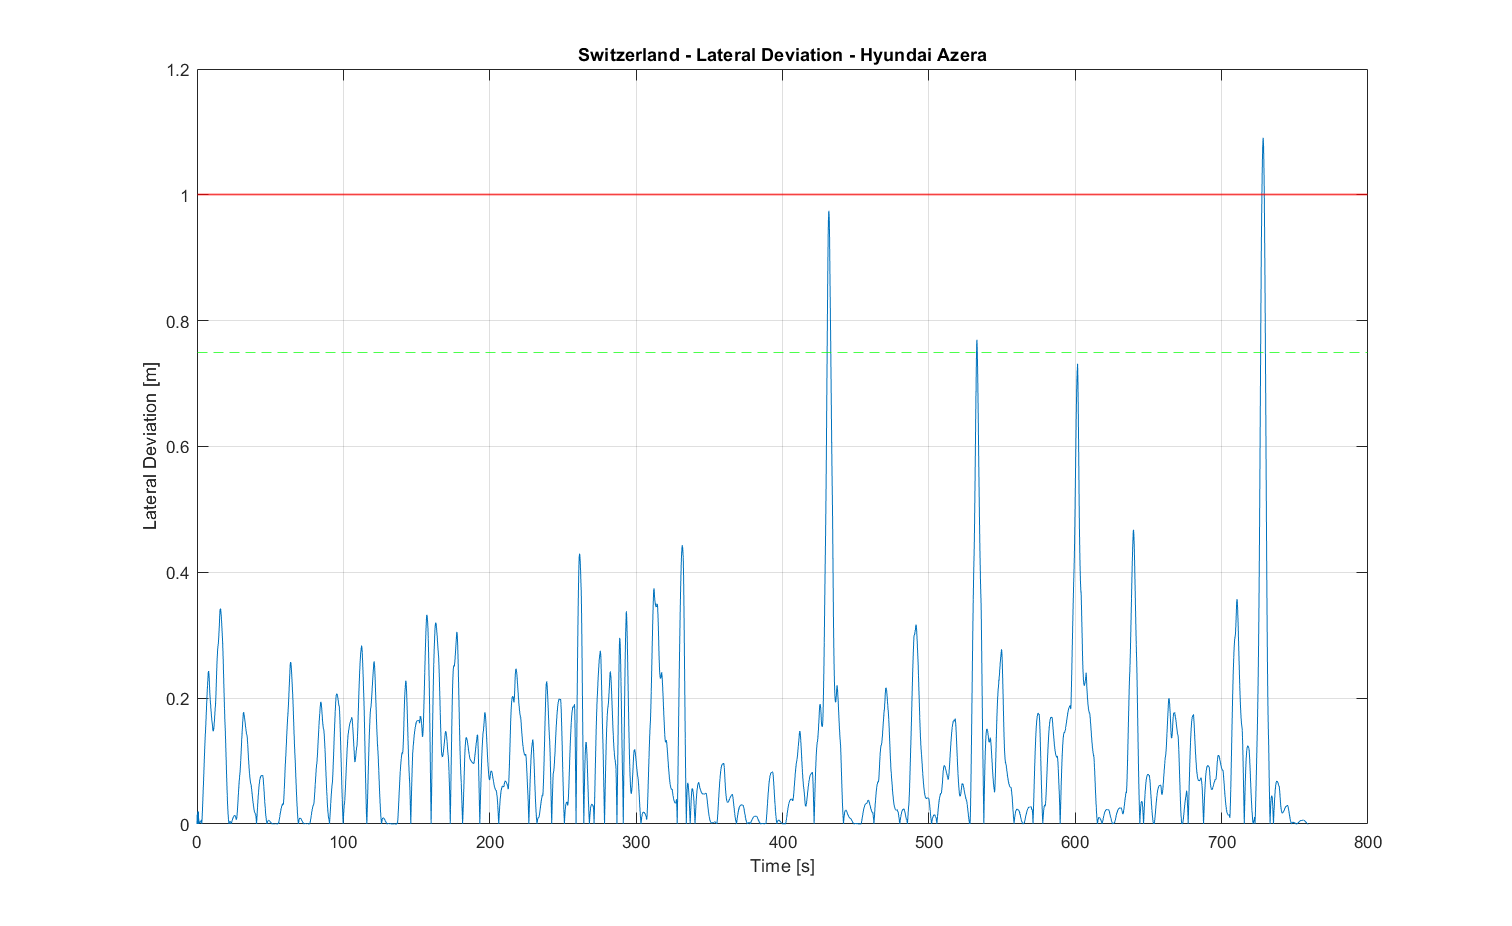
\includegraphics[width=0.95\textwidth,keepaspectratio]{Figures/Switzerland_lateralDev.png}
    \caption{Lateral Deviation Plot (Switzerland)}
    \label{subfig:Switzerland}
    \end{subfigure}
    \caption{Lateral Deviation Comparison}
    \label{fig:lateral_dev_comparison}
\end{figure}


\subsubsection{Failed Tests Analysis}
In the ``Path\_Following-Test\_Report - Failed Tests" we have included the results of the failed tests. In this section we will describe in more detail the issues we have faced during these tests.
What we want to point out is that in the failed tests, the lateral deviation condition is violated only in some specific points, where the curvature of the reference road is, maybe, too high to be performed at constant speed by the vehicle. We encountered this problem in the \textit{Switzerland} scenario with all vehicles and in the \textit{Campania} scenario only with the vehicle Ford E150, which is a heavy van, and it suffers, as expected, of a higher lateral slip compared with other vehicles.
In the following figures, are reported some details about the test performed with the Hyundai Azera in the \textit{Switzerland} Scenario. The figure \ref{fig:SwitzPass} shows how the vehicle behaves in paths with smooth corners, satisfying the lateral deviation requirement, while the figure \ref{fig:SwitzFail} refers to one of the most critical sections of the map, where can be appreciated how the vehicle goes outside the lane in the apex of the hairpin turn.


    \begin{figure}[H]
    \centering
    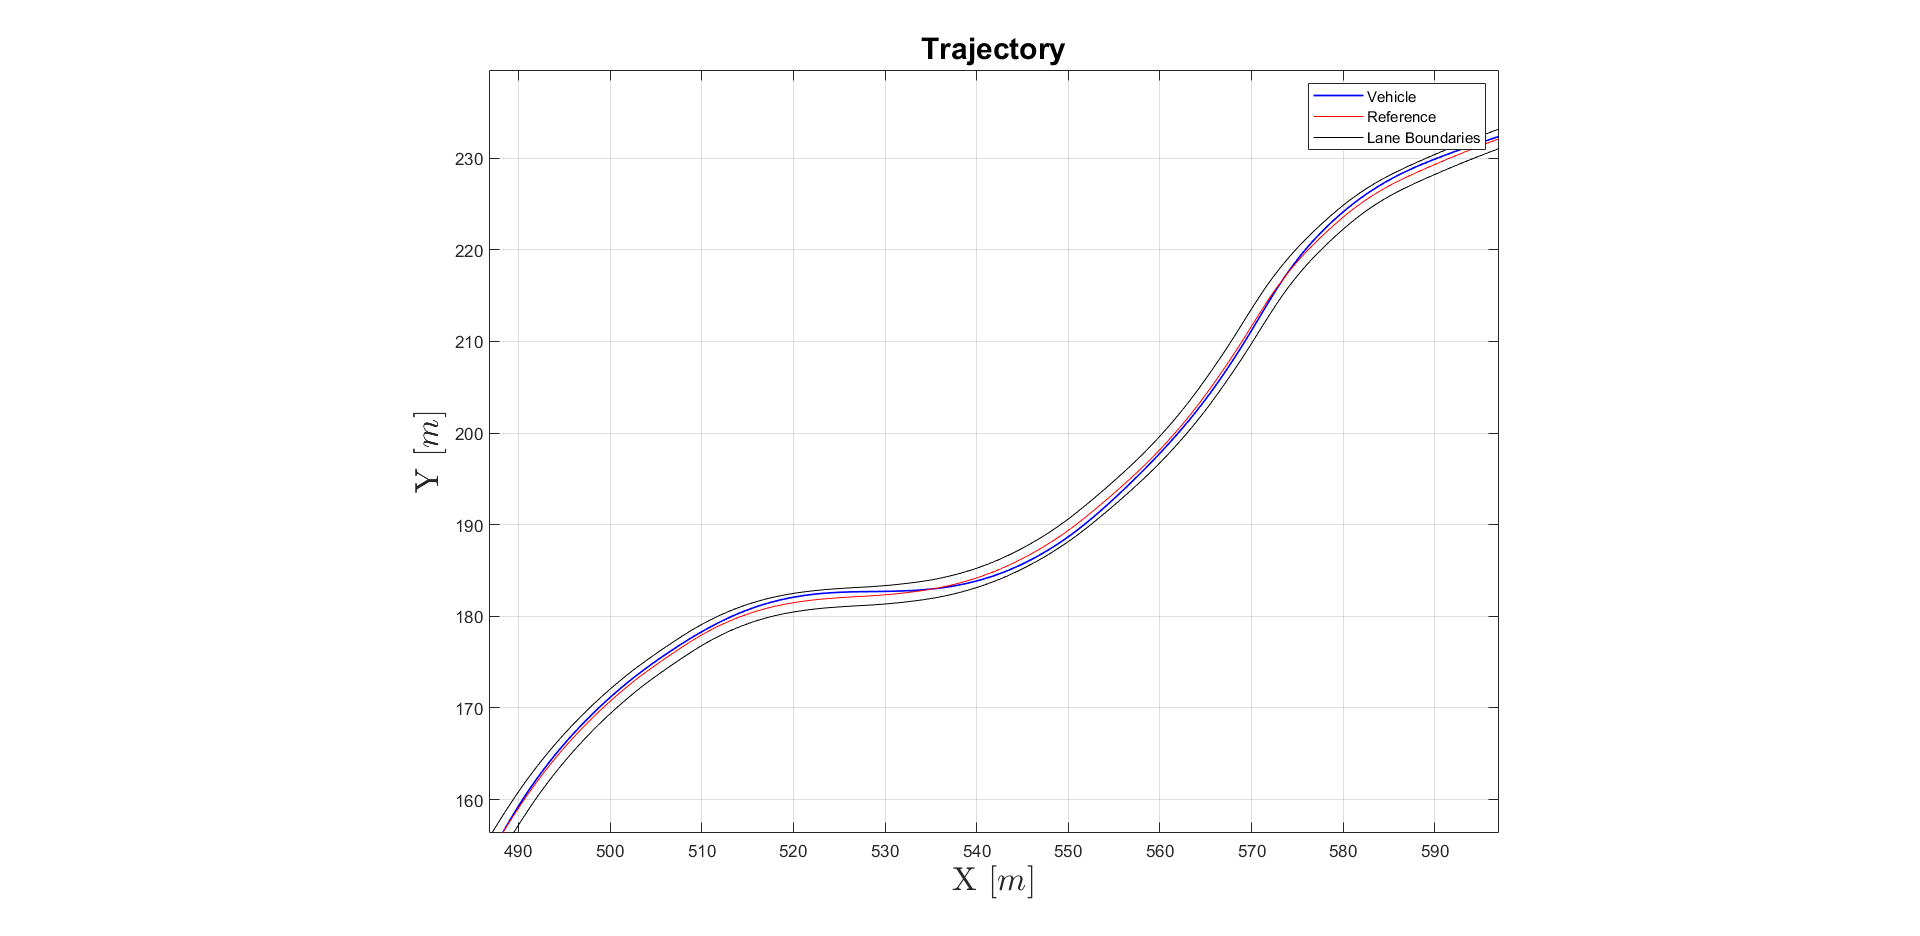
\includegraphics[width=1\textwidth]{Figures/Switz_pass.png}
    \caption{Trajectory of the vehicle in some corners, where all requirements are satisfied}
      \label{fig:SwitzPass}
\end{figure}

    \begin{figure}[H]
    \centering
    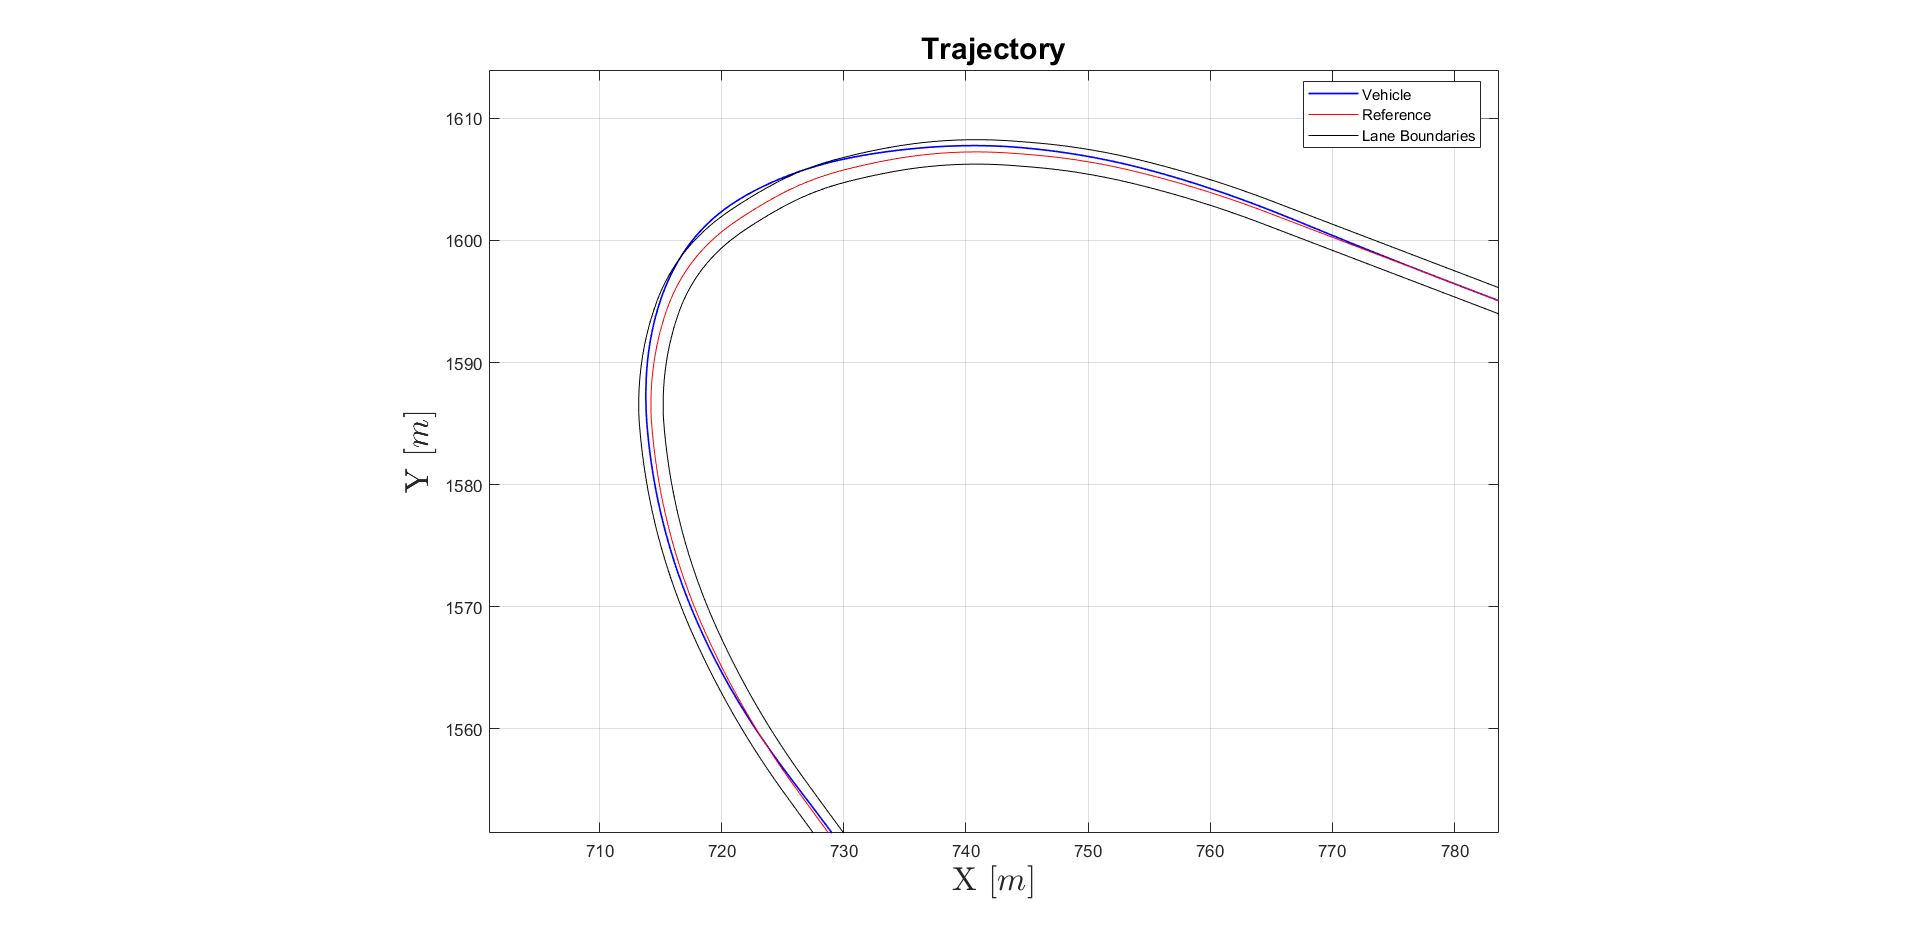
\includegraphics[width=1\textwidth]{Figures/Switz_fail.png}
    \caption{Particular where trajectory of the vehicle is out of the lane boundaries, causing the ``fail" of the test}
      \label{fig:SwitzFail}
\end{figure}


Although these failed tests, we have decided to keep the same controller setup for the obstacle avoidance tests as well, excluding the \textit{Switzerland} Scenario from further simulations.



